\documentclass[a4paper]{book}

%pachete folosite
\usepackage{graphicx}
\usepackage{fullpage}
\usepackage{verbatim}
\usepackage{url}
\usepackage{algorithm}
\usepackage{algpseudocode}
%pachete folosite

%calea catre diagrame
\graphicspath{{diagrams/}}
%calea catre diagrame

%pentru diacritice
\newcommand{\myqq}{''}
\catcode`\'=13
\newcommand{'}[1]{\ifmmode {}^\prime \noexpand#1%
\else\ifx#1a\u{a}% 
\else\ifx#1i\^{i}%
\else\ifx#1s\c{s}% 
\else\ifx#1t\c{t}%
\else\ifx#1j\^{a}%
\else\ifx#1A\u{A}% 
\else\ifx#1I\^{I}%
\else\ifx#1S\c{S}% 
\else\ifx#1T\c{T}%
\else\ifx#1J\^{A}%
\else\ifx#1'\myqq%
	\fi\fi\fi\fi\fi\fi\fi\fi\fi\fi\fi%
\fi}
%pentru diacritice

%titluri in romana 
\def\contentsname{Cuprins}
\renewcommand{\figurename}{Figura}
\renewcommand{\tablename}{Tabelul}
\renewcommand{\chaptername}{Capitolul}
\renewcommand{\bibname}{Bibliografie}
\floatname{algorithm}{Algoritmul}

\newtheorem{thm}{Teorem'a}
%titluri in romana

\mathchardef\mhyphen="2D


\begin{document}


%linie orizontala
\newcommand{\HRule}{\rule{\linewidth}{0.5mm}}
%linie orizontala

%data in format romanesc
\def\today{\space  \ifcase \month
\or IANUARIE\or FEBRUARIE\or mARTIE\or APRILIE\or MAI\or IUNIE\or
IULIE\or AUGUST\or SEPTEMBRIE\or OCTOMBRIE\or NOIEMBRIE\or DECEMBRIE \fi
\space  \number\year}
%data in format romanesc

%pagina de titlu
\begin{titlepage}
\begin{center}
  
%facultatea
\textsc{\LARGE Universitatea Bucure'sti}\\
\textsc{\LARGE Facultatea de matematic'a 'si informatic'a}\\[0.5cm]
\textsc{\Large Specializarea Inteligen't'a Artificial'a}\\[1.5cm]
%facultatea
 

\textsc{\Large Lucrare de diserta'tie}\\[3.0cm]
 
 
%Titlu
\HRule \\[0.5cm]
{ \huge \bfseries Metode de ierarhizare 'in Reg'asirea Informa'tiei}\\[0.4cm]
\HRule \\[4.5cm]
%Titlu
 
%autor si coordonator
\begin{minipage}{0.4\textwidth}
\begin{flushleft} \large
\emph{Autor:}\\
C'alin \textsc{Avas'ilc'ai}
\end{flushleft}
\end{minipage}
\begin{minipage}{0.4\textwidth}
\begin{flushright} \large
\emph{Coordonator:} \\
Lect. Dr. Marius \textsc{Popescu}
\end{flushright}
\end{minipage}
%autor si coordonator
 
\vfill
 
%data curenta
{\large \today}
%data curenta
 
\end{center}
\end{titlepage}
%pagina de titlu

\tableofcontents

\chapter{Introducere}
Singtagma \emph{reg'asirea informa'tiei}(RI) are un spectru larg de in'telesuri. Scoaterea unui card de credit din portofel pentru a completa num'arul cardului 'intr-un formular este o form'a de reg'asire a informa'tiei. Dar, ca domeniu de studii academice, \emph{reg'asirea informa'tiei} poate fi definita astfel\cite{MAN}:
\begin{quote}
Reg'asirea informa'tiei se refer'a la g'asirea de material (de obicei documente) de natur'a nestructurat'a (de obicei text) care satisface
o nevoie de informa'tie, din colectii mari de date (eventual stocate pe calculatoare).
\end{quote}

Reg'asirea informa'tiei obi'snuia s'a fie o activitate practicata de ca'tiva oameni cum ar fi bibliotecarii. Acum lumea s-a schimbat 'si sute de milioane de oameni folosesc sisteme de reg'asire a informa'tiei precum motoate de c'autare web 'in fiecare zi. Reg'asirea informatiei devine rapid forma dominant'a de accesare a informatiei 'intrec'jnd modul tradi'tional de c'autare de tip "baze de date" (c'autarea dupa un num'ar de identificare).

RI este interdisciplinar'a, bazat'a pe informatic'a, matematic'a, 'stiin'ta informa'tiei, arhitectura informa\-'tiei, psihologie cognitiv'a, lingvistic'a, statistic'a, etc. Sisteme automate de RI au fost folosite pentru a reduce ceea ce se numeste "supra'inc'arcarea de informa'tie". Multe universit'a'ti 'si libr'arii publice folosesc sisteme RI pentru a facilita accesul la c'ar'ti, jurnale 'si alte tipuri de documente. Cele mai folosite aplicatii RI sunt motoarele de c'autare web.

\section{Scurt istoric}
Ideea de a folosi calculatoarele pentru a c'auta "buc'a'ti" de informa'tie a fost popularizat'a 'in articolul \emph{As We May Think} de c'atre \emph{Vannevar Bush} 'in anul 1945\cite{IRWIKI}. Primele sisteme automate de reg'asire a informa'tiei au fost introduse 'in anii 1950 si 1960. P'jn'a in 1970 cateva tehnici au fost testate cu succes pe corpusuri mici de text cum ar fi colec'tia \emph{Cranfield} (c'jteva mii de documente). Sisteme mari de RI cum ar fi \emph{Lockheed Dialog system}, au fost date 'in folosin't'a la 'inceputul anilor 1970.

'In 1992 Departamentul de Ap'arare al Statelor Unite 'impreun'a cu Institutul Na'tional de Standarde 'si Tehnologie (NIST) au sponsorizat \emph{TREC} (\textbf{T}ext \textbf{RE}trieval \textbf{C}onference) ca parte din programul TIPSTER. Scopul a fost s'a se asigure comunita'tii RI infrastructura necesar'a pentru testarea 'si evaluarea metodelor de reg'asire a textului pe colectii foarte mari. Acest program a ac'tionat ca un catalizator 'in ceea ce prive'ste cercetarea metodelor RI care scaleaza la colectii foarte mari. Apari'tia motoarelor de c'autare pe web a adus o nevoie si mai mare de sisteme RI care pot face fa'ta unor colec'tii imense de date.

\section{Descrierea procesului}
Un proces de reg'asire a informa'tiei 'incepe c'jnd un utilizator introduce o interogare (\emph{query}) 'in sistem. Interog'arile sunt formul'ari formale ale \emph{nevoilor de informa'tie}, de exemplu, cuvinte scrise 'in caseta de c'autare a unui motor de c'autare web. 'In RI o interogare nu identific'a 'in mod unic un obiect din colec'tia de obiecte. 'In schimb, mai multe obiecte pot fi considerate ca r'aspunsuri la interogare, eventual cu grade de relevan't'a diferite.

Un obiect este o entitate stocat'a 'in sistemul RI. 'In func'tie de aplic'tie, obiectele pot fi texte, documente, imagini, videoclipuri, etc. 'In general, documentele propriu-zise nu sunt 'tinute 'in sistem ci sunt reprezentate de surogate(rezultate 'in urma proces'arii documentelor) si metadate.

Majoritatea sistemelor RI calculeaz'a un scor numeric ce reprezint'a cat de bine se potriveste un obiect cu interogarea utilizatorului 'si apoi ierarhizeaz'a obiectele 'in func'tie de aceast'a valoare. Cele mai bune obiecte sunt apoi afi'sate utilizatorului.

\section{Un exemplu}
%MANNING boolean retrieval 1.1???

\chapter{Reg'asirea informa'tiei - generalit'a'ti}


\section{Procesul de indexare}
\emph{Indexarea} este procesul unui sistem de reg'asire a informa'tiei prin care se colecteaz'a, transform'a, 'si stocheaz'a informa'tia pentru a facilita reg'asirea rapid'a 'si precis'a. Proiectarea unui index presupune cuno'stin'te asupra unor concepte interdisciplinare din lingvistic'a, psihologie cognitiv'a, matematic'a, informatic'a, etc. Motoarele populare de c'autare se concetreaz'a pe indexarea de tip \emph{full-text} ale documentelor online scrise 'in limbaj natural. Tipurile media(video, audio, imagini) pot fi 'si ele indexate. Motoarele de meta-c'autare refolosesc indec'sii altor servicii f'ar'a s'a stocheze un index local, 'in timp ce sistemele RI cu cache stocheaz'a permanent at'jt indexul c'jt 'si corpusul. Spre deosebire de indec'sii full-text, un index \emph{partial-text} restric'tioneaz'a "ad'jncimea" index'arii pentru a reduce dimensiunea indexului. Unele servicii efectueaz'a procesul de indexare la intervale predeterminate de timp din cauza costurilor de procesare, 'in timp ce alte motoarele de c'autare indexeaz'a con'tinut 'in timp real.

\begin{figure}[ht]
    \centering
    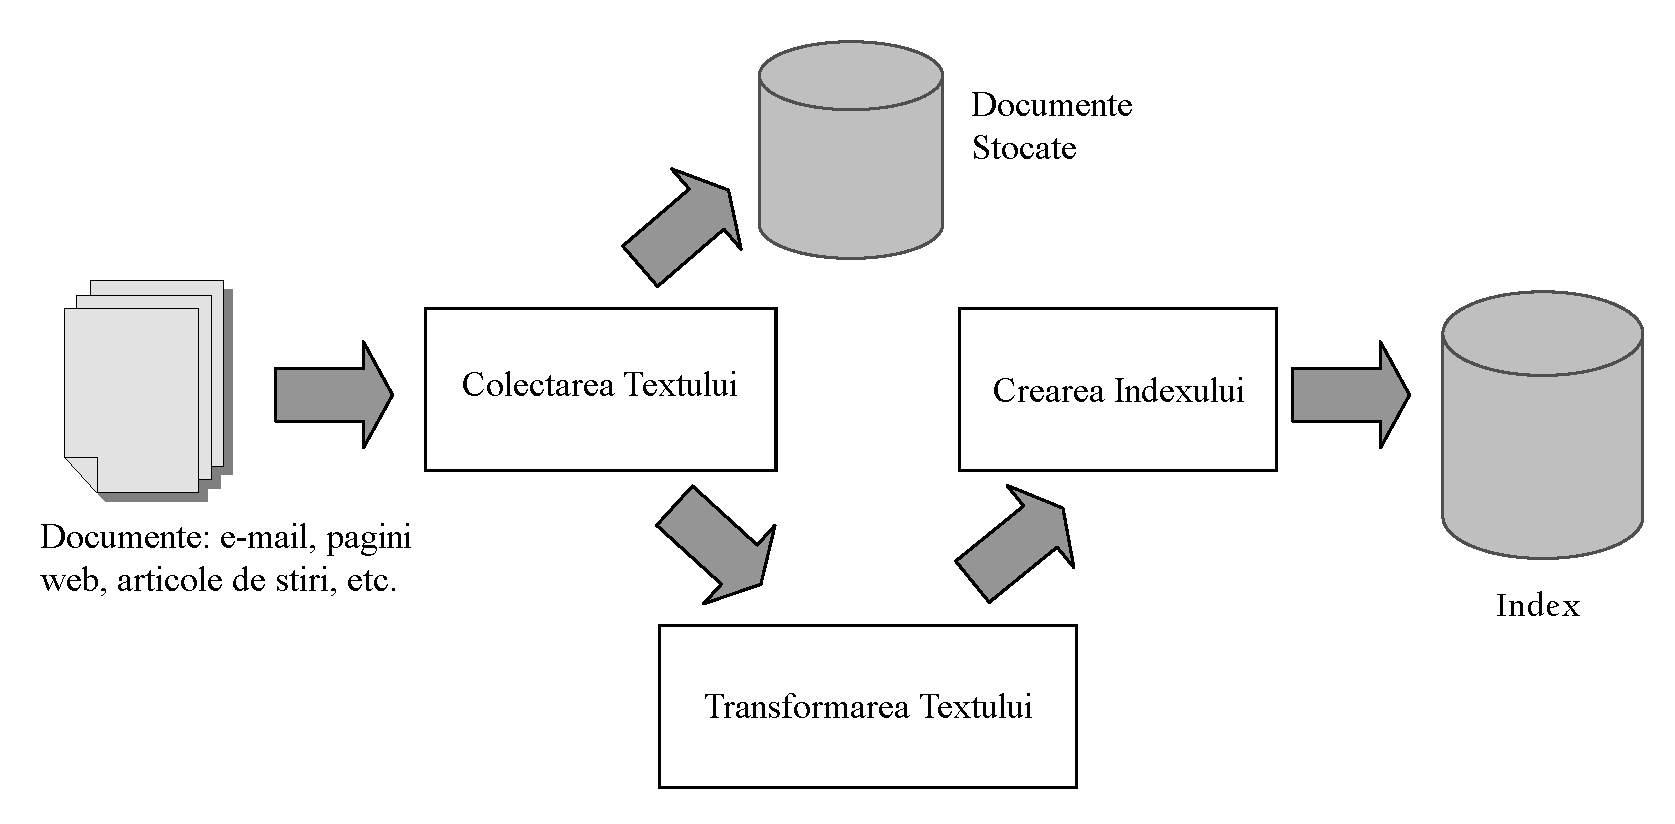
\includegraphics[scale=.25]{ind.png}
    \caption{Indexarea}
    \label{fig:ind}
\end{figure}

\subsection{Colectarea textului}
Una din principalele tehnici prin care un sistem RI colecteaz'a textul pentru indexare este procesul de \emph{crawl-ing}. Un \emph{crawler} indentific'a si ob'tine documente pe care motorul de c'autare le va indexa. Exist'a mai multe tipuri de \emph{crawler-e}: \emph{web, enterprise 'si desktop}. Crawler-ele web urm'aresc hiperleg'aturile dintr-un document pentru a g'asi alte documente. Ele trebuie s'a furnizeze procesului de indexare un num'ar mare de pagini web, 'si, la eventuala modificare a acestora, trebuie depisteze acest lucru 'si s'a declan'seze reindexarea. Pentru asigurarea c'aut'arii pe un singur site se folosesc crawler-ele de site care restrict'ioneaz'a procesul de crawl-ing la un singur domeniu. Crawler-ele pentru c'autarea de tip enterprise 'si desktop indexeaz'a con'tinut local din sisteme de management de con'tinut (CMS) respectiv harddisk-ul local.
Un alt mod de colectare este reprezentat de \emph{feed-uri}: stream-uri de documente 'in timp real (feed-uri web pentru 'stiri, bloguri, video, radio, tv, etc.). Un standard pentru a transporta aceste feed-uri este RSS care poate furniza procesului de indexare documente XML.

Dup'a ce un document este colectat, 'inainte de indexare, acesta trebuie transformat 'intr-un format consistent de text 'si metadate despre document. De exemplu, un motor de c'autare care suport'a mai multe formate (HTML, XML, Word, PDF), le poate transforma 'inainte de indexare 'intr-un format XML. De asemenea, se adopt'a 'si un standard al encod'arii (de exemplu, UTF-8) pentru noile formate.

Unele sisteme RI stocheaz'a documentele 'intr-un \emph{data store} 'inainte s'a le indexeze. Acest lucru facilitez'a accesul componentelor sistemului la setul de documente.

\subsection{Transformarea textului}
'Inainte de a indexa un document acesta este 'imp'ar'tit 'in \emph{tokeni} (parsat) pentru a identifica elementele structurale din text. Tokenii pot fi mai departe procesa'ti prin diverse procese cum ar fi \emph{filtrarea}, \emph{stemming-ul}, \emph{lematizarea}. Tot 'in acest moment se pot efectua procese precum analiza leg'aturilor, extragerea informa'tiei 'si clasificare.

\subsubsection{Parsarea}
Dat fiind o secven't'a de caractere 'si o unitate de document, token-izarea este procesul de 'imp'ar'tire 'in buc'a'ti numite \emph{"token-i"} 'si, 'in acela'si timp, eliminarea anumitor caractere precum semnele de punctua'tie. Ace'sti token-i sunt numi'ti uneori termeni sau cuvinte, dar este important s'a se fac'a distinc'tia 'intre aceste concepte. Un token reprezint'a instan'ta unei secven'te de caractere 'intr-un anumit document, care sunt grupate 'intr-o unitate semantic'a de care se va 'tine cont la procesare. Un \emph{tip} este clasa tuturor token-ilor care con'tin aceea'si secven't'a de caractere. Un \emph{termen} este un tip (de obicei normalizat) care este inclus 'in dic'tionarul sistemului RI. Termenii sunt str'jns lega'ti de token-ii din text, dar, de obicei, sunt ob'tinu'ti prin aplicarea diferitelor procese de normalizare (de exemplu, 'indep'artarea punctelor din prescurt'ari, eliminarea accentelor 'si diacriticelor sau transformarea tuturor literelor 'in litere mici), stemming 'si lematizare.

'Intrebarea major'a care se pune 'in cadrul pars'arii este: \emph{care sunt token-ii potrivi'ti?} Raspunsul este c'a \emph{acest lucru specific limbii}. A'sadar, limba documentului trebuie cunoscut'a. Identificarea limbajului bazat'a pe clasificatori care folosesc secven'te scurte de caractere drept caracteristici este foarte eficient'a, majoritatea limbilor av'jnd modele distincte de astfel de semn'aturi.

\subsubsection{Filtrarea}
C'jteodat'a, unele cuvinte extrem de frecvente, care au o contribu'tie foarte mic'a 'in a ajuta la g'asirea documentelor pentru o nevoie de informa'tie, sunt excluse total din vocabularul de termeni. Aceste sunt numite \emph{cuvinte de stop sau stop words}. Strategia general'a pentru a alc'atui o astfel de list'a de filtrare este selectarea termenilor cu frecven'te foarte mari 'in colec'tia de documente. Folosirea unei liste de filtrare duce la reducerea semnificativ'a a num'arului de post'ari din index 'si, de multe ori, nu are efecte negative (interog'arile de tip fraz'a exact'a constituie un exemplu in care lista de stop are efecte negative).

Iat'a o list'a de cuvinte de stop pentru limba englez'a:
\begin{quotation}
a, an, and, are, as, at, be, by, from, for, has, he, in, is, it, its, on, of, that, the, to, was, where, will, with
\end{quotation}

Tendin'ta folosirii listelor de stop de-a lungul timpului a sc'azut de la liste foarte mare (200-300 termeni), la liste foarte mici (7-12 termeni), ajung'jndu-se la a nu se folosi deloc. 'In general, motoarele de c'autare web nu folosesc cuvinte de stop ci 'intrebuin'teaz'a statisitici ale limbii pentru tratarea mai bun'a a cuvintelor comune.

\subsubsection{Stemming 'si lematizare}
Documentele folosesc diferite forme ale aceluia's cuv'jtnt, de exemplu: \emph{organizez, organizeaz'a, organiz'jnd}. 'In multe situa'tii pare util ca o c'autare a unuia dintre aceste cuvinte s'a 'intoarc'a documente care folosesc oricare din formele lui.

At'jt scopul \emph{stemming-ului} c'jt 'si al \emph{lematiz'arii} este \emph{reducerea formelor flexionare 'si a formelor derivate cu semantic'a similar'a a unui cuv'jnt la o form'a de baz'a}. De exemplu:
\begin{quote}
am, are, is $\Rightarrow$ be
\end{quote}
\begin{quote}
car, cars, car''s, cars'' $\Rightarrow$ car
\end{quote}

Rezultatul aplic'arii acestui tip de reguli este urm'atorul:
\begin{quote}
the boy''s cars are different colors $\Rightarrow$ the boy car be differ color
\end{quote}

De'si au un scop comun, cele dou'a concepte difer'a prin mijloacele folosite. Stemming-ul se refer'a de obicei la procese euristice folosite pentru a 'indep'arta termina'tiile cuvintelor 'in speran'ta atingerii scopului de cele mai multe ori. Lematizarea 'incearac'a sa ating'a scopul prin mijloace mai "formale", folosind un vocabular 'si analiz'jnd morfologic cuvintele (forma din dic'tionar a unui cuv'jnt poart'a numele de \emph{lem'a}). Confruntate cu secven'ta de caractere \emph{saw}, un proces de stemming ar putea 'intoarce \emph{s}, in timp ce lematizarea ar 'incerca s'a intoarc'a \emph{see} sau \emph{saw} 'in func'tie de rolul cuv'jntului (verb, respectiv substantiv).

Cel mai comun algoritm de stemming 'in englez'a este \emph{algoritmul Porter}. S-a constatat 'in mod empiric faptul c'a este foarte eficient.

\subsection{Crearea indexului}
Scopul index'arii este adunarea de "statistici" despre documente 'si stocarea lor 'intr-o structur'a u'sor accesibil'a. Aceste statistici pot fi, de exemplu, frecvent'a 'si pozi'tiile cuvintelor. De obicei, aceste statistici sunt combinate 'in ponderi precum \emph{tf-idf} (sec'tiunea \ref{sec:tfidf}) folosite 'in de algoritmul de ierarhizare. Tehnica de baz'a a index'arii este \emph{inversiunea}. Aceasta are rolulul de a converti informa'tie de tip document-termen 'in termen-document pentru accesarea rapid'a la interogare. Structura de date folosit'a trebuie s'a fie capabil'a s'a suporte actualiz'ari frecvente. Pentru a minimiza costurile de stocare se utilizeaz'a \emph{compresia} care are ca beneficiu 'si facilitarea folosirii sistemelor de caching (mai mult'a informa'tie poate 'inc'apea 'in memorie).
Structura folosit'a de un sistem RI este \emph{indexul inversat}. Acesta este o structur'a de date care stocheaz'a o mapare de la con'tinut ('in acest caz, cuvinte) la loca'tia acestuia (documente). Date fiind textele $T_0$ = "it is what it is", $T_1$ = "what it is" 'si $T_2$ = "it is a banana", un index inversat are urm'atoarea form'a:
\begin{table}[ht]
\centering
\begin{tabular}{ll}
"a" & $\left[2\right]$\\
"banana" & $\left[2\right]$\\
"is" & $\left[0, 1, 2\right]$\\
"it" & $\left[0, 1, 2\right]$\\
"what" & $\left[0, 1\right]$
\end{tabular}
\caption{Index inversat}
\label{tab:invind}
\end{table}

O c'autare dup'a termenii \emph{"what"}, \emph{"is"} 'si \emph{"it"} ar avea urm'atoarele rezultate:
\[
\left\{0, 1\right\} \cup \left\{0, 1, 2\right\} \cup \left\{0, 1, 2\right\} = \left\{0, 1\right\}.
\]

Pentru acelea'si texte se pot stoca 'si pozi'tiile pe care se g'asesc termenii.
\begin{table}[ht]
\centering
\begin{tabular}{ll}
"a" & $\left[\left(2,2\right)\right]$\\
"banana" & $\left[\left(2,3\right)\right]$\\
"is" & $\left[\left(0, 1\right),  \left(0, 4\right), \left(1, 1\right), \left(2, 1\right)\right]$\\
"it" & $\left[\left(0, 0\right), \left(0, 3\right), \left(1, 2\right), \left(2, 0\right)\right]$\\
"what" & $\left[\left(0, 2\right), \left(1, 0\right)\right]$
\end{tabular}
\caption{Index pozi'tional}
\label{tab:invindpoz}
\end{table}


\section{Procesul de c'autare}

\begin{figure}[ht]
    \centering
    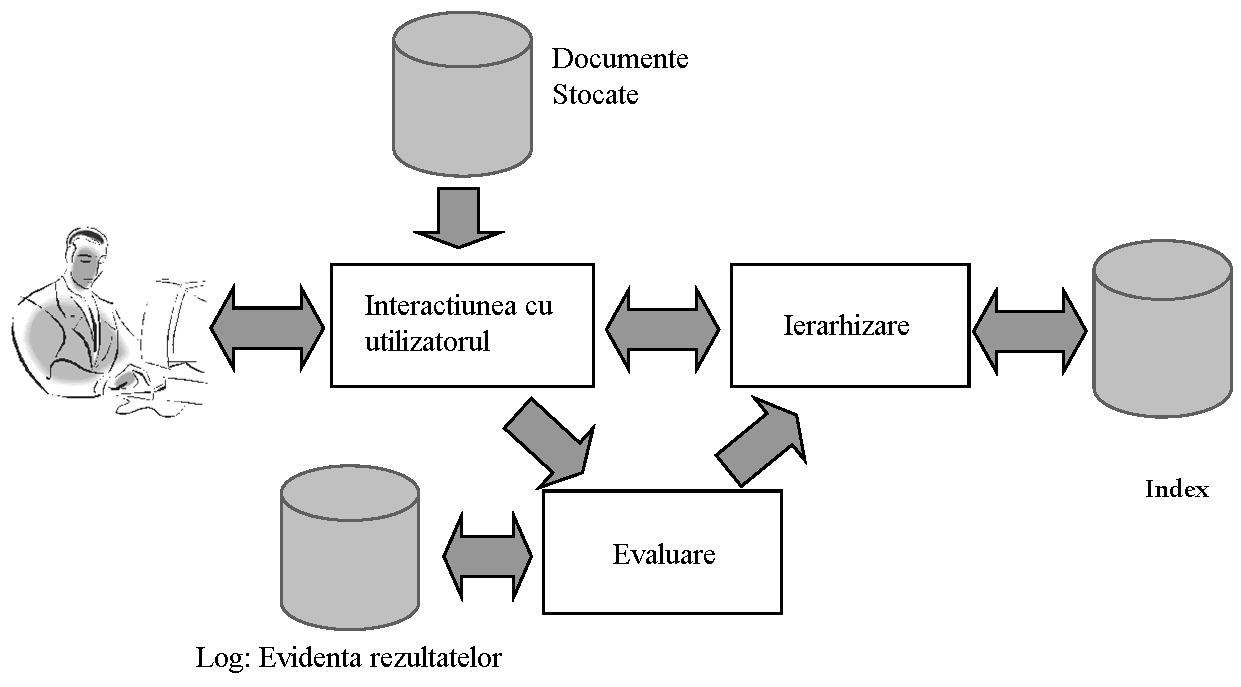
\includegraphics[scale=.34]{quer.png}
    \caption{Interogarea indexului}
    \label{fig:quer}
\end{figure}

\subsection{Interac'tiunea cu utilizatorul}
Un sistem RI pune la dispozi'tia utilizatorului o interfa't'a prin intermediul c'aruia se poate interoga indexul de documente. 'In general, aceast'a interfa't'a este destul de simpl'a, const'jnd 'intr-o caset'a 'in care utilizatorul scrie interogare 'si un buton pentru lansarea c'aut'arii. Interogarea este apoi procesat'a de un parser care interpreteaz'a limbajul folosit. Sintaxa interog'arilor difer'a 'in func'tie de sistem, dar de obicei (mai ales pe web) se folosesc interog'ari de tip free-text 'si eventual c'jtiva operatori logici. Dup'a ce interogarea este trasformat'a intr-o reprezentare intern'a, se aplic'a acelea'si transform'ari ale textului aplicate documentului (filtrare, normalizare, stemming). Unele sisteme verific'a scrierea corect'a 'si pot indic'a sugestii 'in cazul detect'arii erorilor. Pentru a rafina scopul c'aut'arii, un motor de c'autare poate extinde interogarea prin ad'augarea de termeni (sinonime, concepte 'inrudite).

Dup'a ce c'autarea 'si ierarhizarea au avut loc, interfa'ta afi'seaz'a lista de documente. Pentru fiecare document din list'a se afi'seaz'a 'si fragmente 'in care termenii au fost reg'asi'ti (eventual termenii sunt sco'si 'in eviden't'a). Anumite sisteme afi'sez'a 'si reclame relevante la interogarea respectiv'a 'si anumite unelte de vizualizare pentru rafinarea interog'arii sau efectuarea de interog'ari 'inrudite.

\subsection{Procesul de reg'asire 'si ierarhizare}
Algoritmul de ierarhizare poate fi considerat componenta de baz'a a unui sistem de reg'asire a informa'tiei. Strategiile de reg'asire au scopul de a asigna un scor de relevan't'a 'intre o interogare 'si un document. Aceste strategii sunt bazate pe no'tiunea conform c'areia cu c'jt un termen din interogare apare mai des 'in document, cu at'jt este mai "relevant" documentul la interogare. Unele dintre aceste tehnici aplic'a anumite m'asuri care s'a atenueze problemele cauzate de ambiguit'a'tiile limbii (acela'si concept poate fi exprimat folosind termeni diferi'ti sau acela'si termen poate avea sensuri diferite 'in contexte diferite). Un algoritm de ierarhizare are la intrare o interogare $Q$ 'si un set de documente $D_1, D_2, ..., D_n$ iar scopul lui este s'a identifice un coeficient de similaritate $SC(Q, D_i)$ pentru $1 \leq i \leq n$ (SC - \emph{similarity coefficient} - este uneori numit RSV - \emph{retrieval status value}).

Exist'a mai multe modele de reg'asire 'si ierarhizare. O parte din ele sunt ilustrate 'in figura \ref{fig:irm} 'si c'jteva dintre acestea sunt descrise pe scurt 'in paragrafele urm'atoare\cite{GROSS}.

\begin{figure}[ht]
    \centering
    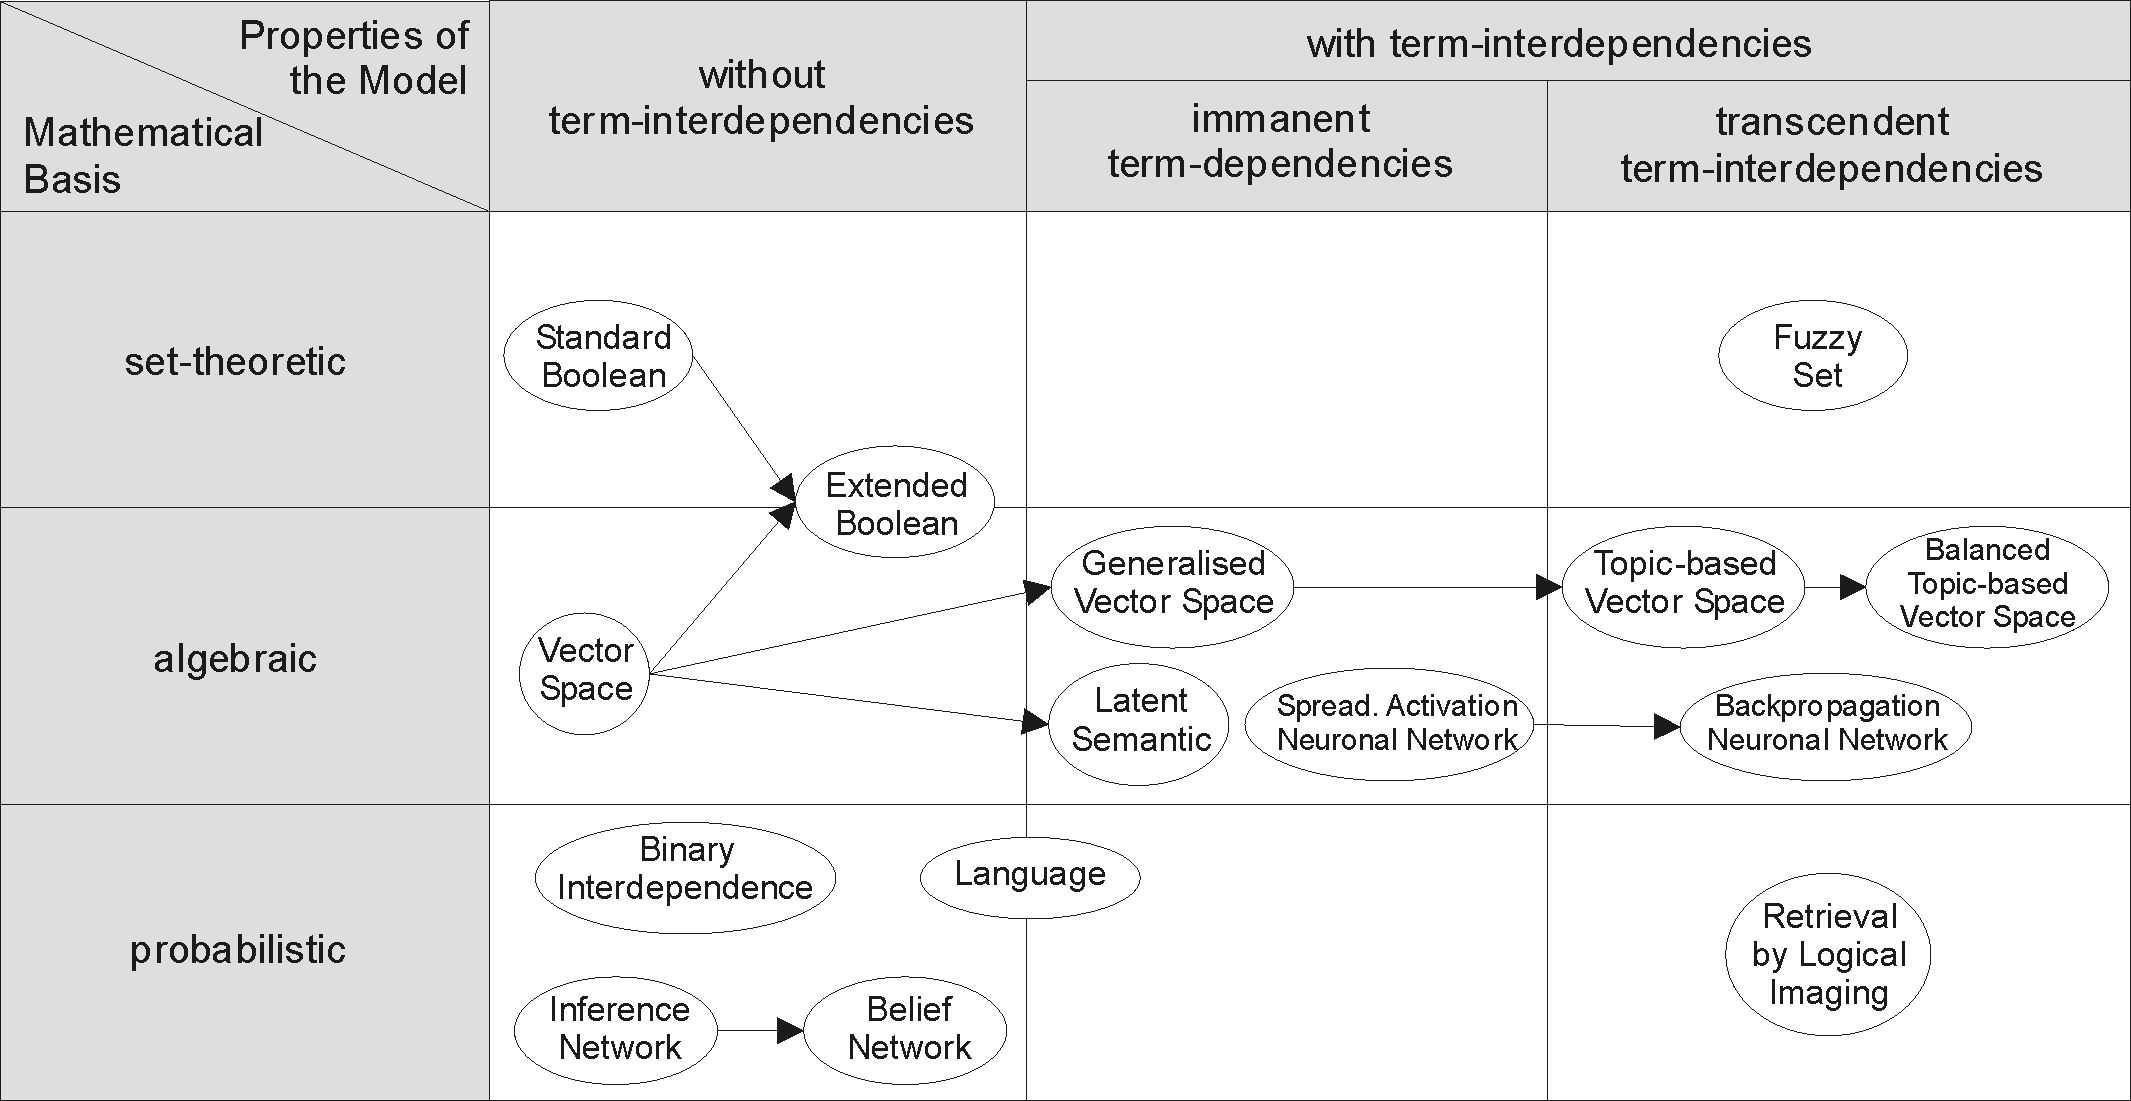
\includegraphics[scale=.8]{irm.png}
    \caption{Diferite modele de ierarhizare clasate dup'a metoda folosit'a 'si modul de tratare a termenilor\cite{IRWIKI}}
    \label{fig:irm}
\end{figure}

\paragraph{Modelul boolean}
La c'autare sunt 'intoarse documentele care satisfac condi'tia logic'a impus'a de interogare 'si, de obicei, se 'tine cont doar de apari'tia respectiv lipsa unui termen din document, nu 'si de frecven't'a.

\paragraph{Modelul spa'tiului vectorial}
'In cadrul acestui model, at'jt interogarea c'jt 'si documentele sunt reprezentate ca vectori 'intr-un spa'tiu vectorial cu c'jte o dimensiune pentru fiecare termen din colec'tie. O m'asur'a de similaritate este calculat'a 'intre interogare 'si un document ca un produs scalar 'intre cei doi vectori normaliza'ti, sau o varia'tiune a acestuia.

\paragraph{Reg'asirea probabilistic'a}
Pentru fiecare termen din colec'tie este calculat'a probabilitatea ca acesta s'a apar'a 'intr-un document relevant. Similaritatea dintre un document 'si o interogare este computat'a ca o combina'tie a probabilit'a'tilor termenilor comuni.

\paragraph{Modele lingvistice}
Un model lingvistic este calculat pentru fiecare document 'si, la c'autare, se calculeaz'a probabilitatea ca un document s'a genereze interogarea.

\paragraph{Re'tele de inferen't'a}
O re'tea baiesian'a este folosit'a pentru a infera relvan'ta unui document la o interogare. Acest'a concluzie se trage pe baza "eviden'telor" din document.

\paragraph{Indexarea semantic'a latent'a}
Ocuren'tele termenilor 'in documente sunt reprezentate folosind o matrice \emph{termen-document}. Matricea este redus'a prin SVD (\emph{Singular Value Decomposition}) pentru a filtra "g'al'agia" (\emph{noise}) g'asit'a 'in documente astfel 'inc'jt dou'a documente care au semantici similare s'a fie situate c'jt mai aproape 'intr-un spa'tiu multi-dimensional.

\paragraph{Re'tele neurale}
Anumi'ti "neuroni" dintr-o secven't'a (noduri 'intr-o re'tea) sunt activa'ti de o interogare 'si produc leg'aturi c'atre documente. "Puterea" fiec'arei leg'aturi din re'tea este transmis'a documentului 'si colectat'a pentru a forma un coeficient de similaritate 'intre interogare 'si document. Re'telele sunt antrenate prin ajustarea ponderilor leg'aturilor pe colec'tii cu interog'ari 'si r'aspunsuri predeterminate.

\paragraph{Algoritmi genetici}
O interogare optim'a pentru a g'asi documente relevante la o nevoie de informa'tie poate fi generat'a prin evolu'tie. O interogare ini'tial'a este folosit'a cu ponderi aleatoare sau estimate ale termenilor. Noi interog'ari sunt generate prin modificarea acestor ponderi. O nou'a interogare "supravie'tuie'ste" dac'a este similar'a cu documentele care se s'tiu a fi relevante la nevoia de informa'tie (predeterminate).

\paragraph{Reg'asirea pe mul'timi fuzzy}
Un document este mapat la o mul'time fuzzy (o mul'time 'in care fiecare element are asociat un num'ar care indic'a "puterea de apartenen't'a"). Interog'arile boolene sunt mapate la intersec'tii, reuniuni 'si complemente de mul'timi fuzzy care au ca rezultat o pondere de apartenten't'a asociat'a cu fiecare document care e relevant la interogare. Aceast'a pondere este folosit'a ca m'asur'a de similaritate.

Pentru fiecare strategie se pot folosi diferite utilit'a'ti sunt folosite pentru a-i imbun'at'a'ti rezultatele. Acestea pot fi: \emph{expandarea interog'arilor}, \emph{feedback-ul de relevan't'a}, \emph{clustering}, \emph{n-grame}, \emph{re'tele semantice}, etc. 'Incerc'jnd s'a rafineze interogarea, majoritatea acestor utilit'a'ti adaug'a sau 'indep'arteaz'a termeni de la interogarea ini'tial'a. Aceste utilit'a'ti sunt componente \emph{"plug-and-play"} 'in sensul c'a ar trebui s'a poat'a fi folosite cu orice model de ierarhizare.

O tratare mai detaliat'a a c'jtorva dintre aceste metode se va face 'in capitolul \ref{cap:rankmet}.

\subsection{Evaluarea}
Pentru 'imbun'at'a'tirea eficien'tei sistemului este crucial'a stocarea interog'arilor 'si interac'tiunilor 'intr-un log. Analiza eficien'tei ierarhiz'arii permite ajustarea sistemului pentru a da rezultate c'jt mai relevante la nevoile de informa'tie 'si constituie o tem'a de baz'a a acestei lucr'ari. Tehnicile de evaluare sunt descrise 'in capitolul \ref{cap:eval}.

\chapter{Evaluarea 'in reg'asirea informa'tiei}
\label{cap:eval}
Exist'a multe alternative pentru a proiecta un sistem RI. Cum hot'ar'jm care dintre aceste tehnici sunt eficiente 'in anumite aplica'tii? Este idicat'a folosirea unui \emph{stop list} sau a unui \emph{stemmer}? Reg'asirea informa'tiei a evoluat ca o disciplin'a empiric'a, necesit'jnd evalu'ari atente 'si complete pentru a demonstra superioritatea performan'telor noilor tehnici ap'arute pe colec'tii reprezentative de documente.
\section{Evaluarea unui sistem RI}
Pentru a m'asura eficien'ta unui sistem ad-hoc RI este necesar'a o colec'tie de test alc'atuit'a din trei componente:
\begin{enumerate}
	\item O colec'tie de documente
	\item O serie de \emph{nevoi de informa'tie} exprimate prin interog'ari
	\item Un set de judec'a'ti de relevan't'a, de obicei o valoare binar'a (\emph{relevant/nerelevant}) pentru fiecare pereche interogare-document.
\end{enumerate}
Abordarea standard 'in evaluarea unui sistem RI se 'inv'jrte 'in jurul no'tiunii de documente \emph{relevante} 'si \emph{nerelevante}. Cu privire la o nevoie de informa'tie, unui document dintr-o colec'tie de test i se d'a o clasificare binar'a: relevant sau nerelevant. Colec'tia de documente 'si setul de interog'ari trebuie s'a fie destul de mari: este nevoie de efectuarea unei medii a rezultatelor de performan't'a peste seturi mari de test 'intruc'jt acestea variaz'a destul de mult de la interogare la interogare. Ca o regul'a derivat'a din experimente, 50 de nevoi de informa'tie reprezint'a un minim suficient.

Relevan'ta este evaluat'a relativ la nevoia de informa'tie, nu la interogare. De exemplu, o nevoie de informa'tie ar putea fi:
\begin{quote}
Informa'tie cu privire la faptul c'a vinul ro'su este mai eficient 'in prevenirea atacurilor de cord dec'jt vinul alb.
\end{quote}
Interog'area asociat'a acestei nevoi de informa'tie ar putea fi:
\begin{quote}
vin 'SI ro'su 'SI alb 'SI atac 'SI cord 'SI eficient
\end{quote}
Un document este relevant dac'a se adreseaz'a nevoii de informa'tie nu doar pentru c'a se 'intampl'a s'a con'tin'a cuvintele din interogare. Acest lucru este des ne'in'teles 'in practic'a, deoarece nevoia de informa'tie este "ascuns'a". 'In orice caz, ea este prezent'a. Pentru o interogare care const'a 'intr-un cuv'jnt, este foarte greu pentru un sistem RI s'a 'i'si dea seama care este nevoia de informa'tie. Dar utilizatorul are o astfel de nevoie 'si va judeca rezultatele pe baza acesteia. Pentru a evalua un sistem este nevoie de o exprimare "deschis'a" a nevoii de informa'tie, care poate fi folosit'a la judecarea documentelor 'intoarse de sistem ca relevante sau nerelevante. Relevan'ta poate fi g'jndit'a ca o scal'a, cu unele documente \emph{mai} relevante dec'jt altele. Dar, pentru 'inceput, se va folosi o valoare binar'a a relevan'tei.

Multe sisteme con'tin diferi'ti parametri de calibrare ce pot fi ajusta'ti pentru a m'ari performan'ta. Este gre'sit s'a se raporteze rezultate pe o colec'tie de test ob'tinute 'in urma modific'arii acestor parametrii cu scopul de a maximiza perfrorman'ta pe colec'tia respectiv'a deoarece parametrii vor fi seta'ti s'a maximizeze performan'ta pe un anumit set de interog'ari 'in loc s'a fac'a acest lucru pentru un e'santion aleator de interog'ari.

\section{Colec'tii sandard de test}
Aceasta este o list'a de colec'tii standard de test si evaluare. Majoritatea sunt menite pentru a testa sisteme ad-hoc de RI dar sunt si c'jteva folosite pentru clasificare de text.
\paragraph{\emph{Cranfield}}
Aceast'a colec'tie a fost prima care a permis m'asuri precise de eficient'a ale sistemelor de reg'asire a informa'tiei, dar acum este prea mic'a pentru un experiment "serios". A fost alc'atuit'a 'in anii 1950 in Regatul Unit 'si con'tine 1398 de sumare de articole despre aerodinamic'a, un set de 225 de interog'ari 'si judec'a'ti de relevan't'a complete pentru toate perechile (interogare, document).
\paragraph{\emph{TREC}}
NIST a construit un framework de evaluare pentru RI 'incep'jnd cu 1992. Din acest framework cele mai cunoscute sunt cele folosite la testele \emph{TREC Ad Hoc track} 'in timpul primelor opt conferin'te TREC (\textbf{T}ext \textbf{RE}trieval \textbf{C}onference) 'intre 1992 'si 1999. 'In total, aceste colec'tii de test 'insumeaz'a 6 CDuri 'si con'tin 1,89 milioane de documente (compuse cu preponderen't'a din articole de 'stiri) 'si judec'a'ti de relevan't'a pentru 450 de nevoi de informa'tie numite subiecte. Colec'tiile TREC 6-8 sunt formate din 150 de nevoi de informa'tie si 528.000 de articole de 'stiri. Acesta este probabil cea mai bun'a subcolec'tie datorit'a faptului c'a este cea mai mare 'si subiectele sunt mai consistente. Din cauza faptului c'a aceste colec'tii sunt foarte mari, nu exist'a judec'a'ti exhaustive ci sunt specificate doar pentru un subset de documente (primele \emph{k} documente 'intoarse de sistemul pentru care nevoia de informa'tie a fost dezvoltat'a).
\paragraph{GOV2}
'In ultimii ani, NIST a f'acut evalu'ari pe colec'tii mult mai mari, incluz'jnd colec'tia de 25 de milioane de pagini web, \emph{GOV2}. GOV2 este acum cea mai mare colec'tie de pagini web disponibil'a pentru cercetare. Cu toate acestea, GOV2 'inc'a este de cel pu'tin 2 ori mai mic'a dec'jt colec'tia de documente indexate de companiile mari de c'autare web.
\paragraph{NTCIR}
Proiectul \emph{NTCIR - NII Test Colections for IR Systems} a construit diferite colec'tii de test de m'arimi similare cu colec'tiile TREC. Aceste colec'tii sunt concentrate pe limba est-asiatic'a 'si pe \emph{reg'asirea informa'tiei cross-language} (interog'arile sunt f'acute 'intr-o limb'a peste un set de documente scrise 'in diferite limbi).
\paragraph{CLEF}
Seria de evalu'ari CLEF (Cross Language Evaluation Forum) s-a concentrat pe limbile europene 'si reg'asirea informa'tiei de tip cross-language.
\paragraph{Reuters}
Pentru clasificarea de text, cea mai folosit'a colec'tie de test a fost \emph{Reuters-21578} compus'a din 21578 articole de 'stiri. Mai recent Reuters a publicat \emph{Reuters Corpus Volume 1 (RCV1)}, o colec'tie mult mai mare const'jnd 'n 806.791 documente.

\section{Evaluarea rezultatelor neordonate}
Av'jnd aceste ingrediente, cum este m'asurat'a eficien'ta unui sistem? Cele mai frecvente si fundamentale dou'a m'asuri 'in RI sunt a'sa-numitele \emph{precizia(precision - P)} 'si \emph{returnarea(recall - R)}. Acestea sunt mai 'int'ji definite pentru cazul 'in care sistemu RI 'intoarce un set neordonat de documente pentru o interogare 'si apoi extinse la liste ierarhizate de documente.

\emph{Precizia} este dat'a de raportul dintre documentele reg'asite care sunt relevante 'si documentele reg'asite:
\begin{equation}
P = \frac{\#(documente\,reg\breve{a}site\,si\,relevante)}{\#(documente\,reg\breve{a}site)} = P(relevante|reg\breve{a}site)
\label{eq:prec}
\end{equation}
\emph{Returnarea} este raportul dintre documentele reg'asite care sunt relevante 'si documentele relevante:
\begin{equation}
R = \frac{\#(documente\,reg\breve{a}site\,si\,relevante)}{\#(documente\,relevante)} = P(reg\breve{a}site|relevante)
\label{eq:rec}
\end{equation}
Aceste no'tiuni pot fi explicate mai clar folosind tabelul de contingen't'a de mai jos.
\begin{table}[ht]
\centering
\begin{tabular}{|l|l|l|}
	\hline
	& Relevante & Nerelevante\\
	\hline
	Reg'asite & pozitive adev'arate(tp) & pozitive false(fp)\\
	\hline
	Nereg'asite & negative false(fn) & negative adev'arate(tn)\\
	\hline
\end{tabular}
\label{tab:relnrel}
\end{table}

Atunci:
\begin{equation}
P = \frac{tp}{tp + fp}\,\,\,\,\,\,\,\,R = \frac{tp}{tp + fn}
\label{eq:precrec}
\end{equation}

O alternativ'a evident'a este judecarea sistemului dup'a acurate'te, adic'a, procentul clasific'arilor corecte. Folosind tabelul de mai sus, $ac = (tp+tn)/(tp+fp+fn+tn)$. Acest lucru pare plauzibil din moment ce exist'a dou'a clase, relevant 'si nerelevant, iar un sistem RI poate fi privit ca un clasificator pe dou'a clase ('intoarce documentele etichetate cu \emph{relevant}). Aceasta este, de fapt, m'asura de eficien't'a folosit'a de obicei 'in evaluarea problemelor de clasificare.

\begin{figure}[ht]
	\centering
	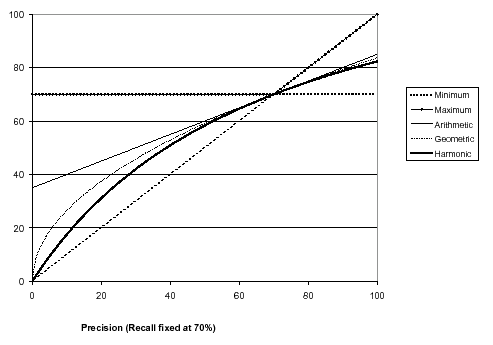
\includegraphics[scale=.7]{evl1.png}
	\caption{Grafic care compar'a media armonic'a cu celelalte medii}
	\label{fig:harm}
\end{figure}

Exist'a un motiv din cauza c'aruia acurate'tea nu este o masur'a corespunz'atoare pentru reg'asirea informa'tiei. 'In aproape toate circumstan'tele, datele sunt extrem de "denaturate": de obicei, peste 99,9\% din documente sunt 'in categoria nerelevant. Un sistem configurat s'a maximizeze acurate'tea poate p'area c'a func'tioneaz'a foarte bine prin considerearea tuturor documentelor ca fiind nerelevante la orice introgare. Acest lucru este inacceptabil pentru un sistem RI. Un utilizator va dori 'intotdeauna s'a vad'a niste documente 'si poate avea o mic'a toleran't'a pentru pozitive false dac'a majoritatea documentelor 'ii satisfac nevoia de informa'tie. M'asurile P 'si R concentreaz'a evaluarea pe 'intoarcerea de pozitive adev'arate, 'intreb'jnd ce procent de documente relevante a fost g'asit 'si cate pozitive false au fost 'intoarse.

Avantajul faptului c'a exist'a dou'a masuri diferite este acela c'a 'in cele mai multe circumstan'te una este mai important'a dec'jt cealalt'a. Un utilizator web obi'snuit dore'ste ca fiecare rezultat de pe prima pagin'a s'a fie relevant(precizie mare) dar nu are nici cel mai mic interes s'a 'stie 'si mai ales s'a priveasc'a fiecare document relevant. Pe de alt'a parte, un profesionist care caut'a documente 'intr-un sistem RI intern va 'incerca s'a g'asesc'a toate documentele relevante la nevoia lui de informa'tie(returnare mare) 'si va tolera valori mici ale preciziei pentru a 'isi atinge scopul. 'In orice caz, exist'a un compromis 'intre cele dou'a valori: se poate 'intotdeauna ob'tine un recall maxim dar precizie mic'a dac'a se 'intorce o list'a cu toate documentele. Recall-ul este o functie non-descresc'atoare de num'arul de documente reg'asite. Pe de alt'a parte, 'intr-un sistem bun, precizia de obicei scade odat'a cu cresterea num'arului de documente reg'asite. 'In general se dore'ste o anumit'a valoare a recall-ului, toler'jndu-se un anumit procent de pozitive false.

O m'asur'a care 'inglobeaz'a at'jt precizia c'jt 'si returnarea este \emph{m'asura F}, care se calculeaz'a ca media armonic'a ponderat'a a celor dou'a valori:
\begin{equation}
F = \frac{1}{\alpha\frac{1}{P} + (1-\alpha)\frac{1}{R}} = \frac{(\beta^2+1)PR}{\beta^2P+R}\,\,\,unde\,\,\,\beta^2=\frac{1-\alpha}{\alpha}
\label{eq:fms}
\end{equation}
unde $\alpha \in [0,1]$ 'si, ca urmare, $\beta^2 \in [0,\infty)$. M'asura F balansat'a 'tine cont 'in mod egal de precizie 'si recall($\alpha=1/2, \beta=1$). Este notat'a de obicei cu $F_1$ (de la $F_{\beta=1}$):
\begin{equation}
F_{\beta=1} = \frac{2PR}{P+R}
\label{eq:f1}
\end{equation}
Valori ale lui $\beta$ mai mici dec'jt 1 scot 'in eviden't'a precizia, 'in timp ce valori mai mari ca 1 pun accentul pe returnare. Valorile discutate p'jn'a acum sunt m'asuri 'intre 0 'si 1, dar se mai scriu si ca procente pe o scal'a de la 1 la 100. Media armonic'a este folosit'a 'in locul mediei aritmetice deoarece 'in cazul 'in care un sistem ar 'intoarce toate documentele(100\% recall), ar avea tot timpul cel pu'tin $F=50\%$. Media armonic'a a dou'a numere ($a << b$) este mai apropiat'a de minim dec'jt de media lor aritmetic'a(vezi figura \ref{fig:harm}).

\section{Evaluarea rezultatelor ordonate}
M'asurile \emph{precision}, \emph{recall} 'si \emph{F} sunt bazate pe seturi; sunt calculate folosind seturi neordonate de documente. Este nevoie de o extindere a acestor m'asuri (sau de o definire de noi m'asuri) dac'a se dore'ste evaluarea unor rezultate ierarhizate care reprezint'a standardul 'in zilele noastre. 'Intr-un context de reg'asire ierarhizat'a setul care intereseaz'a este dat de \emph{primele k} documente. Pentru fiecare astfel de set, valorile preciziei si return'arii pot fi reprezentate grafic printr-o \emph{curb'a precision-recall}, ca cea din figura \ref{fig:precrec}.

\begin{figure}[ht]
	\centering
	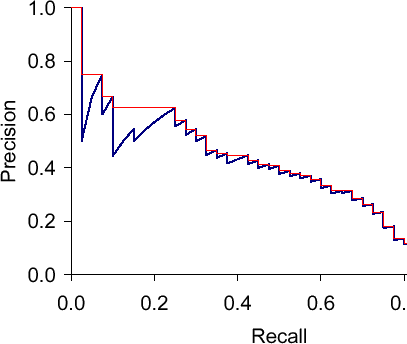
\includegraphics[scale=.7]{evl2.png}
	\caption{Grafic \emph{precision-recall}.}
	\label{fig:precrec}
\end{figure}

Curbele precision-recall au o form'a de "fier'astr'au": dac'a al $(k+1)$-lea document reg'asit este nerelevant, atunci recall-ul este acela'si ca pentru primele $k$ documente reg'asite, dar precizia scade. Dac'a documentul este relevant atunci ambele valori cresc. Este de obicei util s'a se elimine aceast'a form'a 'si modul standard de a face acest lucru este folosind \emph{precizia interpolat'a} $p_{interp}$. La un anumit nivel de recall $r$, $p_{interp}$ este dat de cea mai mare valoare a preciziei g'asit'a pentru orice nivel de recall $r' \geq r$:
\begin{equation}
p_{interp} = \max\limits_{r\prime \geq r}{p(r')}
\label{eq:pinterp}
\end{equation}
Precizia interpolat'a este ilustrat'a 'in figura \ref{fig:precrec}.

Examinarea 'intregii curbe precizion-recall este foarte informativ'a, dar, c'jteodata este necesar ca informa'tia s'a fie redus'a la c'jteva numere. Modul tradi'tional de a realiza acest lucru (folosit, de exemplu, la primele 8 evaluari TREC Ad Hoc) este \emph{precizia medie interpolat'a 'in 11 puncte}. Pentru fiecare nevoie de informa'tie, precizia interpolat'a este m'asurat'a 'in cele 11 puncte de recall: $0.1, 0.2, ..., 1.0$. Exemplul din figur'a \ref{fig:precrec} este ilustrat 'in tabelul \ref{tab:precrec}.
\begin{table}[ht]
\centering
\begin{tabular}{rr}
	Recall & Precizie interpolat'a\\
	0.0 & 1.00\\
	0.1 & 0.67\\
	0.2 & 0.63\\
	0.3 & 0.55\\
	0.4 & 0.45\\
	0.5 & 0.41\\
	0.6 & 0.36\\
	0.7 & 0.29\\
	0.8 & 0.13\\
	0.9 & 0.10\\
	1.0 & 0.08\\
\end{tabular}
\caption{Calcularea preciziei medii interpolate 'in 11 puncte.}
\label{tab:precrec}
\end{table}

Pentru fiecare nivel de recall se calculeaz'a media aritmetic'a a preciziei interpolate la acel nivel de recall pentru fiecare nevoie de informa'tie din colec'tie. O curb'a precizie-recall cu 11 puncte poate fi vizualizat'a apoi grafic. Un exemplu este prezent 'in figura \ref{fig:pinterp}.

\begin{figure}[ht]
	\centering
	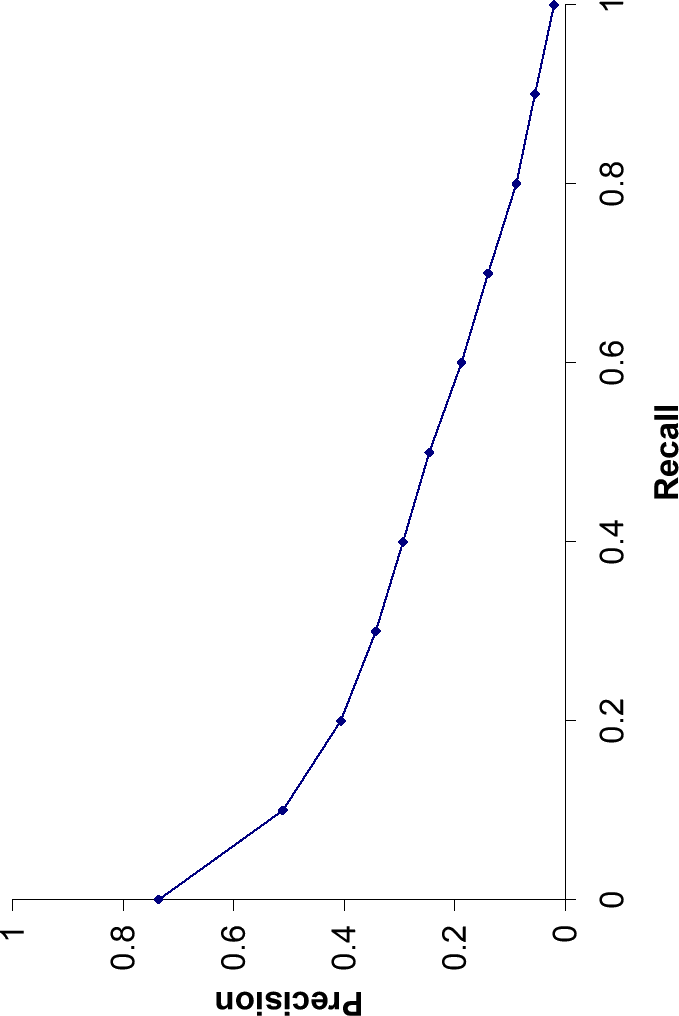
\includegraphics[scale=.4]{evl3.png}
	\caption{Grafic al preciziei medii interpolate 'in 11 puncte.}
	\label{fig:pinterp}
\end{figure}

'In ultimii ani, alte m'asuri au devenit mai comune. Cea mai folosit'a 'in comunitatea TREC este \emph{Mean Average Precision (MAP)}, care pune la dispozi'tie o singur'a m'asur'a de calitatea de-a lungul nivelelor de recall. Printre tipurile de masuri de evaluare s-a ar'atat c'a MAP func'tioneaz'a foarte bine la capitolele discriminare 'si stabilitate. Pentru o sigur'a nevoie de informa'tie, precizia medie este media valorilor de precizie ob'tinute pentru primele \emph{k} documente dup'a reg'asirea fiec'arui document relevant. Media acestei valori peste toate nevoile de informa'tie este MAP. Dac'a setul de documente relevante pentru o nevoie de informa'tie $q_j \in Q$ este ${d_1, ..., d_{m_j}}$ 'si $R_{jk}$ este setul de rezultate de la primul p'jn'a la documentul $d_k$, atunci:
\begin{equation}
MAP(Q) = \frac{1}{|Q|} \sum\limits_{j=1}^{|Q|}{\frac{1}{m_j} \sum\limits_{k=1}^{m_j}{Prec(R_{jk})}}
\label{eq:map}
\end{equation}
C'jnd un document relevant nu este reg'asit, precizia este considerat'a 0. Pentru o singur'a nevoie de informa'tie, precizia medie aproximeaz'a aria de sub curba neinterpolat'a precizie-recall, 'asadar MAP aproximeaz'a aria medie de sub curba precizie-recall pentru un set de interog'ari.

Folosind MAP, nu sunt alese nivele fixe de recall 'si nu este nevoie de interpolare. Un set de nevoi de informa'tie trebuie sa fie cuprinz'ator si diversificat pentru a putea m'asura c'jt mai exact eficient'a unui sistem.

M'asurile descrise p'jn'a au 'in componen'ta precizia pentru fiecare nivel de recall. 'In cazul multor aplica'tii, cum ar fi un motor de c'autare web, acest lucru nu reflect'a neap'arat nevoile unui utilizator. 'In acest caz conteaz'a mai mult c'jte rezultate bune se gasesc 'in primele pagini. Acest lucru conduce la nevoia de a m'asura precizia pentru primele documente reg'asite (10 sau 30). Aceast'a tehnic'a poart'a numele de \emph{"Precizia la k"}. Are avantajul c'a nu necesit'a o esitmare a dimenisiunii setului de documente relevante($m_j$ 'in cazul MAP) 'si dezavantajele c'a este cea mai pu'tin stabil'a dintre metodele de evaluare 'si c'a nu se poate calcula media prea bine pentru ea.

O alternativ'a care atenueaz'a aceast'a problem'a este \emph{R-precizia}. Implic'a existen'ta unui set $Rel$ de documente despre care se 'stie c'a sunt relevante, din care se calculeaz'a apoi precizia pentru primele $|Rel|$ documente reg'asite. R-precizia se ajusteaz'a la m'arimea setului de documente relevante: un sistem perfect ar putea puncta 1 la aceast'a m'asur'a pentru fiecare interogare, 'in timp ce p'jn'a 'si un sistem perfect, ar putea s'a ating'a o precizie la 20 de 0.4 dac'a ar exista doar 8 documente 'in colec'tia de documente relevante. Calcularea mediei peste setul de interog'ari are mai mult sens 'in acest caz. Dac'a exist'a $|Rel|$ documente relevante pentru o interogare, se examineaz'a primele $|Rel|$ rezultate date de un sistem 'si se g'asesc $r$ documente relevante, atunci precizia ('si deci R-precizia) este $r/|Rel|$, dar 'si recall-ul este tot $r/|Rel|$. A'sadar, R-precizia este identic'a cu o alt'a m'asur'a folosit'a c'jteodat'a: \emph{break-even point}, m'asur'a definit'a ca valoarea la care precizia 'si recall-ul sunt egale. Ca 'si \emph{Precizia la k}, \emph{R-precizia} descrie un singur punct de pe curb'a, 'si e uneori neclar de ce intereseaz'a mai mult nivelul 'in care cele dou'a valori sunt egale dec'jt nivelul cel mai bun de pe curb'a ('in care F este maxim) sau un nivelul de interes pentru o anumit'a aplica'tie (\emph{Precizia la k}). Cu toate acestea, R-precizia pare s'a fie corelata cu MAP, lucru constatat 'in urma experimentelor.

Un alt concept folosit uneori 'in evaluarea unui sistem este \emph{curba ROC} ("ROC" vine de la \emph{Receiver Operating Characteristics}). O curb'a ROC reprezint'a grafic rata pozitivelor adev'arate (\emph{senzitivitate}) ca func'tie de rata pozitivelor false (1 - \emph{specificitate}). Aici senzitivitate este un alt terment pentru recall. Rata de pozitive false este dat'a de $fp/(fp+tn)$. Figura \ref{fig:roc} ilustreaz'a cuba ROC corespondent'a cubei precizie-recall din figura \ref{fig:precrec}.

\begin{figure}[ht]
	\centering
	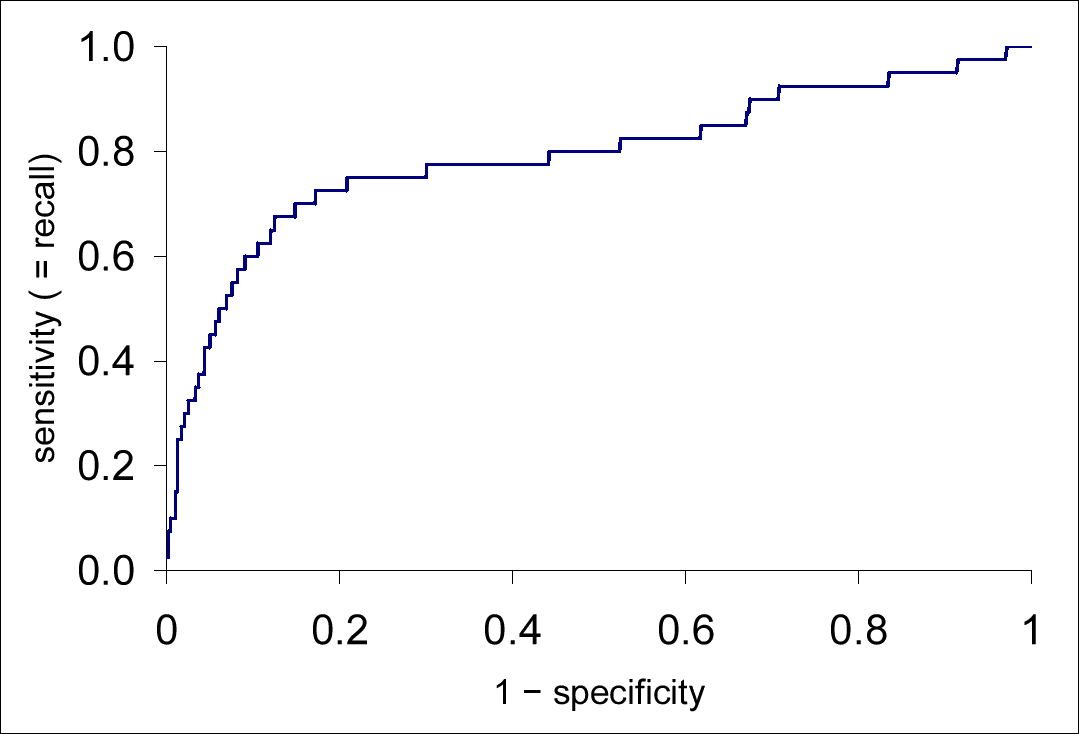
\includegraphics[scale=.4]{evl4.png}
	\caption{Curba ROC}
	\label{fig:roc}
\end{figure}

O curb'a ROC urc'a 'intotdeauna din st'jnga jos spre dreapta sus. Pentru un sistem bun, graficul urc'a abrupt 'in partea st'jng'a. Are mai mult sens c'jnd se ia 'in considerare 'intreg spectrul de reg'asire 'si pune la dispozi'tie o alt'a perspectiv'a asupra datelor. 'In unele cazuri se foloseste estimarea ariei de sub curba ROC, care este o valoare analoag'a m'asurii MAP.

O alt'a abordare care a fost adoptat'a din ce 'in ce mai des, 'in special 'in cazul sistemelor care folosesc \emph{machine learning}, este m'asura \emph{c'j'stigului cumulativ} (\emph{cumulative gain}) 'si, 'in particular, \emph{normalized discounted cumulative gain(NDCG)}. NDCG este proiectat pentru situa'tii 'in care relevan'ta este nebinar'a. Ca 'si \emph{Precizia la k}, este evaluat'a peste primele k rezultate. Pentru un set de interog'ari Q, fie $R(j,d)$ scorul de relevan't'a pe care evaluatorii l-au dat documentului d pentru interogarea j. Atunci,
\begin{equation}
NDCG(Q,k) = \frac{1}{|Q|}\sum\limits_{j=1}^{|Q|}{Z_{kj} \sum\limits_{m=1}^k{\frac{2^{R(j,m)}-1}{\log_2{(1+m)}}}},
\label{eq:ndcg}
\end{equation}
unde $Z_{kj}$ este un factor de normalizare calculat pentru a face ca NDCG-ul unei ierarhiz'ari perfecte la k pentru interogarea j s'a fie 1. Pentru interog'ari pentru care $k' < k$ documente sunt returnate, ultima sum'a se face p'jn'a la $k'$

\chapter{Metode de ierarhizare}
\label{cap:rankmet}
\section{Modelul spa'tiului vectorial (VSM)}
\subsection{Frecven'ta termenilor si ponderarea}
Spre deosebire de o interogarea boolean'a, o interogare \emph{liber'a}("free text") e definit'a de un set de cuvinte neconectate de operatori. Acest tip de interogare este foarte popular'a pe web. Un mecanism de scor pentru aceast'a situa'tie poate fi calcularea sumei dintre scorurile pe care le ob'tine fiecare termen din interogare cu un document.

'In acest scop, se asigneaz'a fiec'arui termen din document o pondere care depinde de num'arul de ocuren'te ale termenului 'in document. Se vrea calcularea unui scor 'intre termenul unei interog'ari, $t$ 'si un document $d$, pornind de la ponderea lui $t$ 'in $d$. Cea mai simpl'a abordare este ca ponderea s'a fie chiar frecven'ta termenului 'in document. Aceast'a schem'a de ponderarea este numit'a \emph{term frequency} 'si notat'a $tf_{t,d}$.

Pentru un docunment $d$, setul de ponderi \emph{tf}(sau orice alte ponderi care mapeaz'a frecven'ta termenilor la numere reale pozitive) poate fi v'azut ca o reprezentare a documentului. 'In acest perspectiv'a asupra unui document, cunoscut'a 'in literatur'a sub numele de \emph{modelul bag of words}, ordinea cuvintelor 'in document este ignorat'a, dar, spre deosebire de modelul boolean, se 'tine cont de frecven'ta lor. 'In orice caz, pare intuitiv faptul c'a dou'a documente care au reprezent'ari similare, sunt similare 'si 'in con'tinut.

O alt'a dilem'a care apare este urm'atoarea: toate cuvintele dintr-un document sunt la fel de importante? 'In mod evident, nu. Pe l'jng'a conceptul de \emph{cuvinte de stop} - cuvinte care nu se indexeaz'a, 'si ca urmare nu contribuie la calcularea scorului - exist'a alt mecanism pentru a c'jnt'ari importan'ta cuvintelor: \emph{frecven'ta invers'a documentelor pentru un termen} sau \emph{idf - inverse document frequency}. 

\subsection{Frecven'ta invers'a a documentelor pentru un termen}
Problema cu ponderarea \emph{tf} este c'a unii termeni ar trebui s'a aib'a mai pu'tin'a putere de discriminare dec'jt al'tii 'in determinarea relevan'tei. Este nevoie de un mecanism care s'a atenueze efectul termenilor care au o frecven'ta mare la nivel de colec'tie. O prim'a idee este reducerea ponderii \emph{tf} a unui termen cu un factor propor'tional cu frecven'ta la nivel de colec'tie(num'arul de ocuren'te 'in toate documentele).

\begin{table}[ht]
\centering
\begin{tabular}{|l|l|l|}
	\hline
	Cuv'jnt & cf & df\\
	\hline
	try & 10422 & 8760 \\
	insurance & 10440 & 3997 \\
	\hline
\end{tabular}
\caption{Frecven'ta la nivel de colec'tie(cf) 'si frecven'ta documentelor(df) se comport'a diferit - exemplu din colec'tia \emph{Reuters}}
\label{tab:dfcf}
\end{table}
'In loc de acest factor, se folose'ste de obicei frecven'ta documentelor $df_t$, definit'a ca num'arul de documente care con'tin termenul $t$. Tabelul \ref{tab:dfcf} ilustreaz'a motivul pentru care este preferat $df$. 'In mod intuitiv, vrem ca pu'tinele documente care con'tin \emph{insurance} s'a aib'a un scor mai mare fa't'a de restul pentru o interogare ce con'tine cuv'jntul \emph{insurance}. Evident, acela'si lucru nu este valabil 'si pentru \emph{try}.

Not'jnd cu $N$ num'arul de documente dintr-o colec'tie, definim frecven'ta invers'a a documentelor pentru un termen $t$, $idf_t$ astfel:
\begin{equation}
idf_t = \log{\frac{N}{df_t}}
\label{eq:idf}
\end{equation}

A'sadar idf-ul unui termen rar este ridicat, 'in timp ce idf-ul unui termen frecvent este sc'azut. Tabelul \ref{tab:dfidf} ilustreaz'a valorile df 'si idf pentru c'j'tiva termeni din colec'tia Reuters.
\begin{table}[ht]
\centering
\begin{tabular}{|l|l|l|}
	\hline
	Termen & $df_t$ & $idf_t$\\
	\hline
	car & 18165 & 1.65\\
	auto & 6723 & 2.08\\
	insurance & 19241 & 1.62\\
	best & 25235 & 1.5\\
	\hline
\end{tabular}
\caption{Exemplu de valori idf din colec'tia Reuters de 806791 documente.}
\label{tab:dfidf}
\end{table}

\subsection{Ponderarea \emph{tf-idf}}
\label{sec:tfidf}
Combin'jnd defini'tiile celor dou'a m'asuri tf 'si idf, se ob'tine o pondere compus'a pentru fiecare temen din fiecare document. Schema de ponderare \emph{tf-idf} asigneaz'a termenului $t$ 'in documentul $d$ dat'a de:
\begin{equation}
tf \mhyphen idf_{t,d} = tf_{t,d} \times idf_t.
\label{eq:tfidf}
\end{equation}

Cu alte cuvinte, $tf \mhyphen idf_{t,d}$ confer'a termenului $t$ din documentul $d$ o pondere care:
\begin{enumerate}
	\item are valorile cele mai mari c'jnd $t$ are un num'ar mare de ocuren'te 'in pu'tine documente
	\item este mai mic'a c'jnd nu apare de foarte multe ori 'in $d$ sau apare 'in multe documente
	\item are valoarea cea mai mic'a (zero) c'jnd apare 'in toate documentele.
\end{enumerate}

'In acest moment fiecare document poate fi vizualizat ca un vector cu c'jte o component'a pentru fiecare termen din dic'tionarul indexului, av'jnd valoarea dat'a de ecua'tia \ref{eq:tfidf}. Aceast'a form'a este crucial'a 'in ierarhizarea 'in RI. O prim'a variant'a de a calcula scorulul unui document 'in raport cu o interogare folosind cele men'tionate p'jn'a acum este:
\begin{equation}
Score(q,d) = \sum\limits_{t \in q}{tf \mhyphen idf_{t,d}}
\label{eq:overlapscore}
\end{equation} 

\subsection{Similaritatea cosinus}
Reprezentarea unui set de documente ca vectori 'intr-un spa'tiu vectorial este cunoscut'a sub numele de \emph{modelul spa'tiului vectorial} (\emph{VSM - vector space model}) 'si este vital'a pentru o serie de opera'tii precum ob'tinerea scorului pentru o interogare, clasificare de documente 'si grupare(\emph{clustering}). Un aspect foarte important al acestui model este reprezentarea interog'arii 'in acel'si spa'tiu vectorial.

\subsubsection{Produsul scalar}
Not'am $\vec{V}(d)$ vectorul derivat din documentul $d$, cu c'jte o component'a pentru fiecare termen din dic'tionar. Presupunem c'a valoarea fiec'arei componente este calculat'a folosind schema de ponderare tf-idf, de'si schema de ponderare este nesemnificativ'a pentru model. Setul de documente din colec'tie poate fi privit acum ca un set de vectori 'intr-un spa'tiu vectorial cu c'jte o ax'a pentru fiecare termen. A'sa cum am mai men'tionat, acest tip de reprezentare ignor'a ordinea termenilor (\emph{bag of words}).

Se pune problema cuantific'arii similarit'a'tii 'intre dou'a documente 'in acest spa'tiu vectorial. O prim'a idee ar fi ca aceasta s'a fie dat'a de vectorul diferen't'a dintre vectorii celor dou'a documente. Problema acestei abord'ari este c'a dou'a documente cu con'tinut similar pot avea o distan't'a foarte mare 'intre ele doar pentru c'a unul este mult mai lung dec'jt cel'alalt, distribu'tia relativ'a a termenilor fiind identic'a (dar frecven'tele absolute diferind).

Pentru a compensa pentru efectul lungimii documentelor, modul standard de a cuantifica similaritatea dintre dou'a documente $d_1$ 'si $d_2$ este calcularea \emph{similarit'a'tii cosinus} ale celor dou'a reprezent'ari vectoriale $\vec{V}(d_1)$ 'si $\vec{V}(d_2)$
\begin{equation}
sim(d_1,d_2) = \frac{\vec{V}(d_1) \cdot \vec{V}(d_2)}{|\vec{V}(d_1)||\vec{V}(d_2)|},
\label{eq:simcos}
\end{equation}
unde num'ar'atorul reprezint'a produsul scalar, 'in timp ce numitorul este produsul lungimilor celor doi vectori. Produsul scalar a doi vectori $\vec{x} \cdot \vec{y}$ este definit ca $\sum_{i=1}^M{x_i y_i}$. Fie $\vec{V}(d)$ reprezentarea vectorial'a a documentului $d$ cu $M$ componente $\vec{V_1}(d), ..., \vec{V_M}(d)$. Lungimea sau norma euclidian'a este definit'a ca $\sqrt{\sum_{i=1}^M{\vec{V_i^2}(d)}}$.

\begin{figure}[ht]
\centering
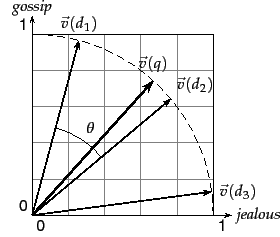
\includegraphics[scale=0.7]{vsm1.png}
\caption{Similaritatea cosinus ilustrat'a pentru interogarea "jealous gossip". $sim(d_1, d_2) = \cos{\theta}$}
\label{fig:simcos}
\end{figure}

Efectul num'aratorilor este, a'sadar, s'a normalizeze vectorii $\vec{V}(d_1)$ 'si $\vec{V}(d_2)$ la vectorii unitate $\vec{v}(d_1) = \vec{V}(d_1)/|\vec{V}(d_1)|$ 'si $\vec{v}(d_2) = \vec{V}(d_2)/|\vec{V}(d_2)|$. Putem rescrie ecua'tia \ref{eq:simcos} ca:
\begin{equation}
sim(d_1,d_2) = \vec{v}(d_1) \cdot \vec{v}(d_2).
\label{eq:simcos1}
\end{equation}

Ecua'tia \ref{eq:simcos1} poate fi v'azut'a ca produsul scalar dintre versiunile normalizate ale vectorilor celor dou'a documente. Aceast'a valoare reprezint'a cosinusul unghiului $\theta$ dintre cei doi vectori (vezi figura \ref{fig:simcos}). Dat fiind un document d, m'asura de similaritate poate fi folosit'a la g'asirea altor documente asem'an'atoare lui d. Acest lucru poate fi dorit de un utilizator care identific'a un document relevant la nevoia lui de informa'tie 'si, pornind de la acest document, dore'ste s'a g'asesc'a alte documente relevante. O astfel de abordare poart'a numele de \emph{mai multe ca acesta - more like this}. Problema g'asirii documentului $d_i$ cel mai asem'an'ator cu $d$ se reduce la g'asirea unui document $d_i$ cu proprietatea c'a produsul scalar $\vec{v}(d) \cdot \vec{v}(d_i)$ este maxim.

Vizualizarea unei colec'tii de N documente ca o colec'tie de vectori conduce la vizualizarea colec'tiei ca o \emph{matrice termen-document}. Aceasta este o matrice de dimensiune $M \times N$ ale c'arei r'jnduri reprezint'a cei M termeni(dimensiuni) ale celor N coloane, fiecare corespunz'jnd unui document.

\subsubsection{Interog'arile v'azute ca vectori}
Exist'a un motiv 'si mai convig'ator pentru reprezentarea documentelor ca vectori: reprezentarea interog'arilor ca vectori. Ideea acum este s'a se asigneze fiec'arui document $d$ din colec'tie un scor egal cu produsul scalar $\vec{q} \cdot \vec{d}$.

Prin vizualizarea unei interog'ari ca "un sac de cuvinte" (\emph{bag of words}), se poate trata ca un document foarte scurt. Scorurile rezultate 'in urma calcul'arii similarit'a'tilor fiec'arui document cu interogarea pot fi apoi folosite pentru a selecta 'si ierarhiza documentele relevante.
\begin{equation}
sim(q,d) = \frac{\vec{V}(q) \cdot \vec{V}(d)}{|\vec{V}(q)||\vec{V}(d)|},
\label{eq:simcosq}
\end{equation}

Un document poate avea un scor cosinus mare pentru o interogare chiar dac'a nu con'tine to'ti termenii din interogare. Formula similarit'a'tii cosinus nu se bazeaz'a pe o anumit'a ponderare a termenilor, schema de ponderare put'jnd fi tf, tf-idf sau alte tipuri sau varia'tiuni.

Calcularea similarit'a'tii cosinus 'intre vectorul interog'arii 'si vectorii fiec'arui document din colec'tie, sortarea sorurilor rezultate 'si selectarea primelor $K$ documente pot fi opera'tiuni costisitoare - computarea unei singure similarit'a'ti poate duce la calcularea unui produs sclalar pentru mii de dimensiuni (num'arul termenilor din colec'tie). De aceea exist'a o serie de euristici folosite pentru a 'imbun'at'a'ti timpul necesar efectu'arii calcului (vezi sec'tiunea \ref{sec:eur}).

\subsubsection{Calcularea scorurilor}
'Intr-o situa'tie uzual'a avem o colec'tie de documente, fiecare reprezentat de un vector, o interogare reprezentat'a de un vector 'si un 'intreg pozitiv $K$. C'aut'am primele K documente din colec'tie cu sorurile date de similaritatea cosinus cele mai mari 'in contextul interog'arii date. De exemplu, multe motoare de c'autare folosesc $K=10$ pentru a reg'asi si ierarhiza documentele afi'sate pe prima pagin'a (cele mai bune). Algoritmul \ref{alg:cossim} prezint'a algoritmul de baz'a pentru computarea scorurilor.

\begin{algorithm}
\caption{Calcularea similarit'a'tii cosinus}\label{alg:cossim}
\begin{algorithmic}[1]
\Procedure{CosineScore}{$q$}\Comment{primele K documente 'in ordinea similatit'a'tii cosinus}

\State float $Scores[N]\gets 0$
\State initialize $Length[N]$

\ForAll{$t \in q$}\label{alg:cossim:1}
	\State calculate $w_{t,q}$\label{alg:cossim:2}\Comment{ponderea termenului t 'in interogarea q}
	\State fetch postings list ${P_t}$ and $idf_t$ for term t
	\ForAll{$(d, tf_{t,d}) \in P_t$}\label{alg:cossim:3}
		\State $wf_{t,d} \gets tf_{t,d} \times idf_t$\Comment{sau orice alt'a schem'a de ponderare}
		\State $Score[d] \gets Score[d] + wf_{t,d} \times w_{t,q}$\Comment{produsul scalar}
	\EndFor
\EndFor
\State read array $Length[d]$\Comment{norma euclidian'a pentru fiecare document}

\ForAll{$d$}
	\State $Scores[d] \gets Scores[d] / Length[d]$\Comment{normalizare}
\EndFor

\State \textbf{return} Top \textbf{K} components of $Scores[]$\label{alg:cossim:4}

\EndProcedure
\end{algorithmic}
\end{algorithm}

Lista $Length$ 'tine lungimile vectorilor (factorii de normalizare) pentru fiecare dintre cele $N$ documente, 'in timp ce lista $Scores$ 'tine scorul fiec'arui document. Dup'a ce scorul este calculat, tot ceea ce r'am'jne de f'acut este s'a se aleag'a primele $K$ documente cu scorul cel mai mare.

Prima bucl'a de la pasul \ref{alg:cossim:1} itereaz'a peste fiecare termen din interogare actualiz'jnd scorul pentru fiecare document. La pasul \ref{alg:cossim:2} se calculeaz'a ponderea termenului $t$ 'in vectorul interog'arii. Itera'tia de la pasul \ref{alg:cossim:3} actualizeaz'a fiecare document din lista de postare a termenului $t$ cu contribui'tia aferent'a. Acest proces este cunoscut sub numele de \emph{acumulare} iar elementele listei $Scores$ sunt \emph{acumulatori}. Pentru a evita stocarea numerelor 'in virgul'a mobil'a 'in index, se poate stoca $df_t$ pentru fiecare termen, 'si $tf_{t,d}$ pentru fiecare document dintr-o list'a de postare. La c'autare, pentru fiecare termen t, se poate calcula $idf_t$ 'si apoi ponderea tf-idf pentru fiecare document din lista de postare. La pasul \ref{alg:cossim:4} sunt extrase primele $K$ documente; acest proces necesit'a o coad'a cu prioritate implementat'a de obicei folosind ca structur'a de date un heap.

Algoritmul \ref{alg:cossim} nu prescrie o implementare specific'a despre cum trebuie traversate listele de postare ale termenilor din interogare. Acestea pot fi traversate pentru fiecare termen 'in parte sau 'in mod concurent, pentru to'ti termenii, calcul'jnd la fiecare pas 'intregul scor al unui document (cu condi'tia ca documentele s'a fie ordonate dup'a acela'si criteriu 'in fiecare list'a). Prima variant'a poart'a numele de \emph{term-at-a-time} iar cea de-a doua, \emph{document-at-a-time}.

\subsection{Variante de ponderare tf-idf}
Au fost propuse 'si alte alternative la \emph{tf} 'si \emph{idf} pentru ponderarea termenilor din documente.

\subsubsection{Scalarea subliniar'a \emph{tf}}
Pare improbabil ca 20 de ocuren'te ale unui termen 'intr-un document au o 'insemn'atate de 20 de ori mai mare dec'jt o singur'a ocuren't'a. Ca urmare, s-au c'autat variante de luare 'in considerare a frecven'tei termenilor folosind func'tii care nu cresc liniar cu num'arul de ocuren'te. O abordare comun'a este folosirea logaritmului frecven'tei termenilor:
\begin{equation}
wf_{t,d} = \left\{
\begin{array}{ll}
	1 + \log{tf_{t,d}} & dac\breve{a} \quad tf_{t,d} > 0\\
	0 & altfel
\end{array}
\right..
\label{eq:logtf}
\end{equation}
Utiliz'and aceast'a pondere 'in loc de tf, putem 'inlocui tf-idf cu:
\begin{equation}
wf-idf_{t,d} = wf_{t,d} \times idf_t.
\label{eq:wfidf}
\end{equation}

\subsubsection{Normalizarea cu tf maxim}
O alt'a tehnic'a este normalizarea ponderilor $tf$ pentru fiecare termen din document cu $tf$-ul maxim din acel document. Fie $td_{max}(d) = \max_{\tau \in d}{tf_{\tau,d}}$ pentru fiecare document $d$. Frecven'ta normalizat'a a termenilor este calculat'a astfel:
\begin{equation}
ntf_{t,d} = a + (1 - a)\frac{tf_{t,d}}{tf_{max}(d)},
\label{eq:ntf}
\end{equation}
unde $a$ este o valoare 'intre 0 'si 1 (de obicei ia valoarea $0.4$) 'si se nume'ste \emph{factor de uniformizare}. Are rolul de a amortiza contribu'tia frac'tiei din ecua'tia \ref{eq:ntf} (ideea de baz'a este s'a se evite o oscila'tie mare a $ntf_{t,d}$ cauzat'a de o oscila'tie mic'a a $tf_{t,d}$).

Ideea principal'a din spatele normaliz'arii cu tf maxim este evitarea urm'atoarei anomalii: se observ'a frecven'te mai mari ale termenilor 'in documente mai lungi, 'in principal din cauza faptului c'a documentele mai lungi tind s'a repete acelea'si cuvinte de mai multe ori, lucru care nu ar trebui s'a afecteze calcularea relevan'tei.

\subsubsection{Scheme de ponderare pentru documente 'si interog'ari}
Ecua'tia \ref{eq:simcosq} este fundamental'a pentru sisteme de reg'asirea informa'tiei care folosesc orice form'a de ierarhizare pe baza VSM. Diferen'tele dintre metodele VSM 'tin mai degrab'a de alegerea ponderilor din vectorii $\vec{V}(d)$ 'si $\vec{V}(q)$. Tabelul \ref{tab:smart} ilustreaz'a unele dintre principalele scheme de ponderare folosite at'jt pentru $\vec{V}(d)$ c'jt 'si pentr $\vec{V}(q)$, 'impreun'a cu mnemonice pentru a reprezenta o combina'tie specific'a de ponderi. Acest sistem de mnemonice poart'a numele de \emph{nota'tia SMART}.

\begin{table}[ht]
\centering
\begin{tabular}{|l|l|l|}
\hline
Frecven'ta termenilor(tf) & Frecven'ta 'in documente & Normalizare\\
\hline
\begin{tabular}{ll}
n & $tf_{t,d}$\\
l & $1 + \log{tf_{t,d}}$\\
a & $0.5 + \frac{0.5 \times tf_{t,d}}{\max_t{tf_{t,d}}}$\\
b & $\left\{\begin{array}{ll}
1 & dac\breve{a} \quad tf_{t,d} > 0\\
0 & altfel
\end{array}\right.$\\
L & $\frac{1+\log{tf_{t,d}}}{1+\log{ave_{t \in d}(tf_{t,d})}}$
\end{tabular}&
\begin{tabular}{ll}
n & 1\\
t & $\log{\frac{N}{df_t}}$\\
p & $\max\left\{0,\,\log{\frac{N-df_t}{df_t}}\right\}$
\end{tabular}&
\begin{tabular}{ll}
n & 1\\
c & $\frac{1}{\sqrt{\sum\limits_{i=1}^M{w_i^2}}}$\\
u & $1/u$\\
b & $1/Cl^{\alpha}, \alpha < 1$
\end{tabular}\\
\hline
\end{tabular}
\caption{Nota'tia \emph{SMART} pentru variantele tf-idf; \emph{Cl} reprezint'a numarul de caractere din document}
\label{tab:smart}
\end{table}

Nota'tia pentru reprezentarea unei combina'tii de scheme de ponderare are forma $ddd.qqq$, unde primul triplet reprezint'a ponderarea pentru vectorul documentului iar cel de-al doilea pentru interogare. Prima liter'a din fiecare triplet reprezint'a componenta frecven'tei termenului, cea de-a doua, frecven'ta 'in documente, iar cea de-a treia, forma de normalizare folosit'a. 'In practic'a, se aplic'a scheme diferite de normalizare pentru document, respectiv interogare. De exemplu, o schem'a de ponderare des 'int'jlnit'a este \emph{lnc.ltc}.

\section{Euristici pentru eficientizare}
\label{sec:eur}
Revizualiz'jnd algoritmul \ref{alg:cossim} pentru o interogare \emph{q = jealous gossip}, dou'a observa'tii sunt imediate:
\begin{enumerate}
\item Vectorul $\vec{v}(q)$ are dou'a componente diferite de zero.
\item 'In absen'ta unei ponder'ari pentru termenii interog'arii, cele dou'a componente nenule au aceea'si valoare.
\end{enumerate}
Pentru a ierarhiza documentele relevante la interogare, suntem interesa'ti de scorurile relative ale documentelor din colec'tie. A'sadar, este suficient'a calcularea similarit'a'tii cosinus 'intre fiecare vector normalizat $\vec{v}(d)$ 'si $\vec{V}(q)$ ('in care toate componentele nenule sunt egale cu 1) 'in loc de $\vec{v}(q)$. Pentru oricare dou'a documente $d_1, d_2$
\begin{equation}
\vec{V}(q) \cdot \vec{v}(d_1) > \vec{V}(q) \cdot \vec{v}(d_2) \Leftrightarrow \vec{v}(q) \cdot \vec{v}(d_1) > \vec{v}(q) \cdot \vec{v}(d_2).
\label{eq:rankeq}
\end{equation}

Pentru fiecare document $d$, similaritatea cosinus $vec{V}(q) \cdot \vec{v}(d)$ este suma peste to'ti termenii din interogarea $q$ a ponderilor acestor termeni 'in $d$. Aceast'a sum'a se poate calcula prin intersectarea listelor de postare ca 'in algoritmul \ref{alg:cossim}, cu men'tiunea c'a ponderile interog'arii sunt considerate 1. Aceast'a schem'a calculeaz'a un scor pentru fiecare document din listele de postare ale termenilor din interogare (num'arul de documente poate fi considerabil mai mic dec'jt $N$).

\begin{algorithm}
\caption{Un algoritm mai rapid pentru calcularea similarit'a'tii cosinus}\label{alg:cossim1}
\begin{algorithmic}[1]
\Procedure{CosineScore}{$q$}\Comment{primele K documente 'in ordinea similatit'a'tii cosinus}

\State float $Scores[N]\gets 0$
\State initialize $Length[N]$

\ForAll{$t \in q$}\label{alg:cossim1:1}
    \State fetch postings list ${P_t}$ and $idf_t$ for term t
    \ForAll{$(d, tf_{t,d}) \in P_t$}\label{alg:cossim1:3}
        \State $wf_{t,d} \gets tf_{t,d} \times idf_t$\Comment{sau orice alt'a schem'a de ponderare}
        \State $Score[d] \gets Score[d] + wf_{t,d}$
    \EndFor
\EndFor
\State read array $Length[d]$\Comment{norma euclidian'a pentru fiecare document}

\ForAll{$d$}
    \State $Scores[d] \gets Scores[d] / Length[d]$\Comment{normalizare}
\EndFor

\State \textbf{return} Top \textbf{K} components of $Scores[]$\label{alg:cossim1:4}

\EndProcedure
\end{algorithmic}
\end{algorithm}

Dup'a calcularea scorurilor, pasul final 'inainte de prezentarea rezultatelor unui utilizator este s'a se aleag'a $K$ documente cu cele mai bune scoruri. Se poate folosi o sortare dar o abordare mai bun'a este folosirea unui \emph{heap} pentru a p'astra ordinea documentelor. Dac'a $J$ este num'arul de documente cu scoruri nenule, construirea acestui heap poate fi f'acut'a 'in $2J$ pa'si.

\subsection{Reg'asirea inexact'a a primelor K documente}
P'jn'a acum scopul primordial a fost reg'asirea \emph{precis'a} a primelor $K$ documente pentru o interogare. 'In continuare voi prezenta scheme cu ajutorul c'arora sunt produse $K$ documente pentru care 'sansele sunt foarte mari s'a fac'a parte din \emph{primele K}. Proced'jnd astfel, scopul este de a mic'sora semnificativ costul reg'asirii, f'ara a altera percep'tia utilizatorului asupra relevan'tei documentelor 'intoarse. 'In sec'tiunile urm'atoare sunt detaliate euristici care realizeaz'a acest lucru.

O astfel de reg'asire inexact'a nu e 'in mod necesar, din perspectiva utilizatorului, un lucru r'au. Documentele din \emph{top-K} dup'a similaritatea cosinus nu sunt neap'arat cele mai bune $K$ pentru nevoia respectiv'a de informa'tie. Principalul cost decurge din calcularea similarit'a'tii cosinus 'intre interogare 'si un num'ar mare de documente. Un num'ar mare de documente duce 'si la cre'stereea costului de selec'tie 'in faza final'a de extragere din heap.

Vom considera, 'in continuare o serie de idei care au ca scop eliminarea unui num'ar mare de documente f'ar'a a mai calcula similaritatea. Euristicile au la baz'a urm'atorii pa'si:
\begin{enumerate}
\item G'ase'ste un set $A$ de documente pretendente, unde $K < |A| << N$. $A$ nu con'tine neap'arat cele mai bune $K$ documente, dar 'sansele sunt foarte mari s'a con'tin'a o bun'a parte din acestea.
\item 'Intoarce cele mai bune $K$ documente din $A$.
\end{enumerate}

Din descrierea acestor idei, este clar c'a multe dintre euristici vor necesita parametri care s'a fie ajusta'ti la colec'tie 'si aplica'tie. Majoritatea acestor euristici sunt adecvate pentru interog'ari de tip "free text" dar nu 'si pentru interog'ari booleane sau "fraz'a exact'a".

\subsection{Ignorarea termenilor}
Pentru o interogare multi-termen $q$, este evident c'a se vor lua 'in calcul doar documente care con'tin cel pu'tin unul din termeni. Acest lucru poate fi extins folosind euristici adi'tionale:
\begin{enumerate}
\item Se consider'a doar documente care con'tin termeni ale c'aror ponderi $idf$ sunt mai mari dec'jt o valoare prestabilit'a. A'sadar, la traversarea listelor de postare, se traverseaz'a doar listele termenilor cu $idf$ mare. Acest lucru aduce un beneficiu mare: listele de postare ale termenilor cu ponderi $idf$ mici sunt 'in general lungi; prin 'indep'artarea lor setul de documente pentru care trebuie calculat'a similaritatea scade considerabil. O alt'a perspectiv'a asupra acestei euristici este c'a termenii cu $idf$ redus sunt considera'ti cuvinte de stop 'si nu contribuie la calcularea scorului.
\item Se consider'a doar documente car con'tin mul'ti (sau to'ti) tereni din interogare. Acest lucru poate fi realizat la traversarea post'arilor. Un pericol al acestei scheme este c'a dac'a se elimin'a prea multe documente setul de documente $A$ va avea mai pu'tin de $K$ documente.
\end{enumerate}

\subsection{Listele de campioni}
Ideea din spatele \emph{listelor de campioni} (\emph{champion lists, fancy lists, top docs}) este precomputarea, pentru fiecare termen $t$ din dic'tionar, unui set de $r$ documente care au ponderi foarte mari pentru $t$; valoare lui $r$ este aleas'a ini'tial. Pentru ponderarea $tf-idf$, acestea ar fi primele $r$ cu ponderea $tf$ cea mai mare pentru termenul $t$. Numim acest'a mul'time de $r$ documente \emph{lista de campioni} a termenului $t$.

Av'jnd o interogare q, cream setul $A$ astfel: lu'am reuniunea listeror de campioni ale fiec'arui termen din $q$. Restric'tion'am calcularea similarit'a'tii cosinus doar la documentele din A. Un parametru critic al acestei scheme este valoarea lui $r$, care variaz'a 'in func'tie de aplica'tie. Intuitiv, $r$ ar trebui sa fie mult mai mare dec'jt $K$, mai ales dac'a se folosesc euristicile prezentate 'in sec'tiunea precendet'a. O problem'a 'in cazul acesta este c'a $r$ este setat'a la construirea indexului, 'in timp ce $K$ este dependent de aplica'tie 'si exist'a posibilitatea s'a fie aflat doar la lansarea interog'arii. Ca urmare, se poate 'intmpla ca setul $A$ sa aib'a mai pu'tin de $K$ documente. Valoare lui $r$ ar putea fi setat'a mai mare pentru termeni mai rari.

\subsection{Scoruri statice}
Extindem listele de campioni la no'tiunea de \emph{scoruri statice}. 'In multe motoare de c'autare pentru fiecare document $d$ este disponibil'a o m'asur'a a calit'a'tii $g(d)$ independent'a de interogare, deci static'a. Aceast'a m'asur'a poate fi privit'a ca o valoare 'intre 0 'si 1. De exemplu, 'in contextul unei 'stiri de pe web, $d(d)$ ar putea fi derivat'a din num'arul de review-uri favorabile primite de la vizitatori.

\begin{figure}[ht]
	\centering
	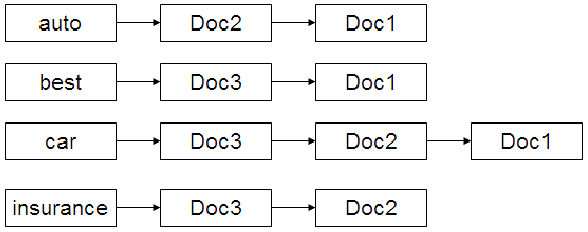
\includegraphics[scale=.7]{stat.png}
	\caption{Index ordonat static. g(1) = 0.25, g(2) = 0.5, g(3) = 1}
	\label{fig:stat}
\end{figure}

Scorul net pentru documentul $d$ este o combina'tie 'intre $g(d)$ 'si scorul calculat la momentul interog'arii dup'a o anumit'a schem'a. Combina'tia poate fi determinat'a printr-un proces de 'inv'a'tare, dar, de dragul simplit'a'tii, vom considera urm'atoarea form'a:
\begin{equation}
score(q, d) = g(d) + \frac{\vec{V}(q) \cdot \vec{V}(d)}{|\vec{V}(q)||\vec{V}(d)|}.
\label{eq:stat}
\end{equation}
'In aceast'a form'a simpl'am scorul static $g(d)$, 'si scorul calculat la interogare au contribu'tii egale, presupun'jnd c'a amblele se afl'a 'intre 0 'si 1.

Mai 'int'ji s'a consider'am ordonarea documentelor din lista de postare a fiec'arui termen 'in mod descresc'ator dup'a valoarea lui $g(d)$. Acest lucru permite efectuarea intersect'arii listelor de postare 'in mod concurent ca 'si cum ar fi fost ordonate dup'a id-ul documentului (e nevoie doar de o ordonare comun'a pentru toate listele de postare). Acest tip de ordonare este ilustrat 'in figura \ref{fig:stat}.

Una dintre idei este extinderea direct'a a listelor de campioni: pentru o valoare bine aleas'a $r$, men'tinem pentru fiecare termen $t$, o list'a de $r$ documente cu valorile cele mai mari ale $g(d) + tdidf_{t,d}$. Lista este sortat'a dup'a o ordonare comun'a. Apoi, la interogare, se calculeaz'a scorul net doar pentru documentele din reuniunea acestor liste de campioni.

Cea de-a doua idee const'a 'in men'tinerea, pentru fiecare termen $t$, a dou'a liste de postare disjuncte, fiecare sortat'a dup'a $g(d)$. Prima list'a, numit'a \emph{high}, con'tine cele $m$ documente cu valorile $tf$ cele mai mari pentru $t$. Cea de-a doua list'a numit'a \emph{low}, con'tine toate celelalte documente ce 'il con'tin pe $t$. C'jnd se proceseaz'a o interogare, se scaneaz'a mai 'int'ji lista \emph{high}, calcul'jnd scorurile nete pentru fiecare document (sau documente care con'tin un num'ar mare din termenii interog'arii). Dac'a nu se ob'tin $K$ documente 'in urma acestui proces, se continu'a cu listele \emph{low}.

\subsection{Impact ordering}
'In toate listele de postare descrise p'jn'a acum, documentele au fost ordonate dup'a o ordonare comun'a (dup'a id-ul documentului sau scoruri statice). O astfel de ordonare comun'a suport'a traversarea concurent'a a listelor de postare, calcul'jnd scorul pentru fiecare document 'in momentul 'in care acesta este 'int'jlnit. O astfel de abordare este numit'a notare \emph{document-at-a-time}. 'In aceast'a sec'tiune voi vorbi despre o tehnic'a 'in care listele de postare nu sunt toate ordonate dup'a o ordonare comun'a, lucru care 'impiedic'a o traversare concurent'a. Ca urmare, scorurile vor fi "acumulate" lu'jnd termenii pe r'jnd ca 'in algoritmul \ref{alg:cossim} (\emph{term-at-a-time}).

Idee const'a 'in ordonarea documentelor din listele de postare descresc'ator dup'a $tf_{t,d}$. Ca urmare, ordonarea va fi diferit'a de la o list'a de post'ari la alta 'si nu se poate face o traversare concurent'a pentru to'ti termenii din interogare. Av'jnd listele ordonate descresc'ator dup'a $tf_{t,d}$, dou'a ideei s-au remarcat 'in a reduce substan'tial num'arul de documente pentru care terbuie acumulate scorurile:
\begin{enumerate}
\item c'jnd se traverseaz'a lista unui termen $t$, algoritmul se opre'ste dup'a ce parcurge un anumit prefix al acesteia - fie dup'a un num'ar fix $r$ de intr'ari, fie dup'a ce $tf_{t,d}$ a sc'azut sub o anumit'a valoare presetat'a;
\item termenii interog'arii se parcurg 'in ordinea descresc'atoare a $idf$, astfel 'inc'jt termenii care au o probabilitate mai mare s'a contribuie mai mult la scorurile finale s'a fie lua'ti 'in considerare primii.
\end{enumerate}
Aceast'a ultim'a idee poate fi adaptat'a la momentul proces'arii interog'arii: c'jnd se ajunge la termeni ai interog'arii cu $idf$ sc'azut, se poate determina dac'a se continu'a pe baza schib'arilor scorurilor documentelor de la parcurgerea listei termenului anterior. Dac'a schimb'arile sunt minime, se poate omite procesarea listei, sau se poate procesa doar un prefix.

Aceste idei vin dintr-o generealizare a metodelor introduse 'in sec'tiunile precedente. Depinz'jnd de metoda de ponderare, listele de postare pot fi ordonate dup'a alte cantit'a'ti dec'jt frecven'ta termenilor. 'In contextul RI aceast'a metod'a poart'a numele de \emph{impact ordering}.

\subsection{Cluster pruning}
'In \emph{cluster pruning} exist'a un etap'a de preprocesare 'in cadrul c'areia vectorii documentelor sunt grupa'ti. Apoi, la momentul interog'arii, se consider'a doar documentele dintr'un num'ar mic de grupuri drept candida'ti pentru care se calculeaz'a similaritatea. Pa'sii de preprocesare sunt urm'atorii:
\begin{enumerate}
\item Alege $\sqrt{N}$ documente din colec'tie 'in mod aleator. Nume'ste aceste documente \emph{lideri}.
\item Pentru fiecare document care nu este lider, afl'a care este cel mai "apropiat" lider.
\end{enumerate}
Documentele care nu sunt lideri vor fi numite \emph{adep'ti}. Intuitiv, num'arul aproximativ de \emph{adep'ti} pentru fiecare lider este $\approx N / \sqrt{N} = \sqrt{N}$. Procesul de interogare decurge 'in felul urm'ator:
\begin{enumerate}
\item Dat'a fiind o interogare $q$, g'ase'ste liderul $L$ cel mai apropiat de $q$. Acest lucru presupune computearea similarit'a'tilor cosinus 'intre $q$ 'si fiecare dintre cei $\sqrt{N}$ lideri.
\item Setul de candida'ti $A$ este alc'atuit din $L$ 'si adep'tii acestuia. Se computeaz'a scorurile pentru toate documente din acest set.
\end{enumerate}

Folosirea liderilor ale'si aleator pentru grupare este rapid'a 'si probabilitatea s'a reflecte distribu'tia vectorilor 'in spa'tiu este destul de mare. Acest luctru este ilustrat 'in figura \ref{fig:cp}.

\begin{figure}[ht]
	\centering
	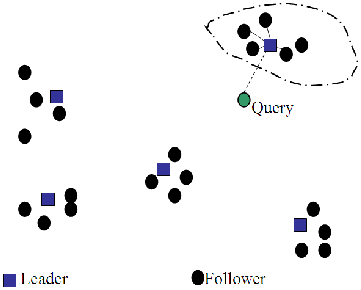
\includegraphics[scale=.7]{cp.png}
	\caption{Cluster pruning}
	\label{fig:cp}
\end{figure}

Varia'tii ale acestei metode introduc parametrii adi'tionali $b_1$ 'si $b_2$, 'intregi pozitivi. 'In faza de preprocesare se ata'sez'a fiecare adept la cei mai apropia'ti $b_1$ lideri. La procesul de c'autare se consider'a cei mai apropia'ti $b_2$ lideri de interogarea $q$. Schema de mai sus corespunde cazului $b_1=b_2=1$. Cre'sterea celor doi parametri duce la cre'sterea 'sanselor de a g'asi $K$ documente care sa fac'a parte din $top-K$, dar necesit'a mai multe computa'tii.


\section{Modelul probabilistic}
Dac'a s-ar cunoa'ste relevan'ta unui subset de documente, s-ar putea estima probabilitatea apari'tiei unui termen \emph{t} 'intr-un document relevant $P(t|R=1)$ 'si, ca urmare, acesta ar putea reprezenta baza unui clasificator care decide dac'a un document este relevant sau nu.

Utilizatorii 'incep cu \emph{nevoi de informa'tie} pe care le transform'a 'in \emph{interog'ari}. 'In mod similar, documentele sunt transformate 'in \emph{reprezent'ari de documente} care difer'a de primele cel pu'tin prin felul 'in care textul este 'imp'ar'tit 'in token-i. Baz'jndu-se pe aceste dou'a reprezent'ari, un sistem 'incearc'a s'a determine c'jt de bine satisfac documentele nevoile de informa'tii. 'In modelul Boolean sau VSM, d'jndu-se numai o interogare, pentru un sistem RI nevoia de informa'tie este incert'a. D'jndu-se interogarea 'si reprezentarea documentelor, un sistem trebuie s'a "ghiceasc'a" daca un document are con'tinut relevant pentru respectiva nevoie de informa'tie. Teoria probabilit'a'tilor pune la dispozi'tie o funda'tie de principii potrivite pentru ra'tionament 'in situa'tii incerte. Aceste principii pot fi exploatate pentru a estima c'jt de probabil este ca un document sa fie relevant pentru o nevoie de informa'tie.

Exist'a mai multe posibile modele probabilistice de reg'asire. 'In continuare voi discuta despre \emph{principiul probabilistic de ierarhizare} 'si despre \emph{modelul binar de independen't'a}, care a fost primul model probabilistic de reg'asire. 'In final voi prezenta 'si sistemul de ponderare \emph{Okapi BM25}, care a avut un succes destul de mare 'in practic'a.

'In acest context, este util conceptul de 'sanse (\emph{odds}), pe l'jng'a cel de probabilitate.
\begin{equation}
Odds: O(A) = \frac{P(A)}{P(\bar{A})} = \frac{P(A)}{1 - P(A)}.
\label{odds}
\end{equation}

\subsection{Principiul probabilistic de ierarhizare}
\subsubsection{Cazul 1/0 loss}
Presupunem c'a sistemul de RI 'intoarce ca r'aspuns la o interogare o list'a ordonat'a de documente 'si folosirea unei nota'tii binare pentru relevan't'a. Pentru o interogare \emph{q} 'si un document \emph{d}, fie $R_{d,q}$ o variabil'a aleatoare care indic'a dac'a \emph{d} este relevant 'in contextul interog'arii \emph{q}. Variabila ia valoarea 1 c'jnd documentul este relevant 'si 0 altfel.

Folosind un model probabilistic, ordinea evident'a 'in care documentele trebuie prezentate utilizatorului este dat'a de ierarhizarea documentelor dup'a probabilitatea estimat'a de relevan't'a 'in raport cu nevoia de informa'tie: $P(R_{d,q}=1|d,q)$. Vom scrie $R$ 'in loc de $R_{d,q}$. Aceasta reprezint'a temelia \emph{principiului probabilistic de ierarhizare (PRP)}:

\begin{quote}
Dac'a r'aspunsul unui sistem la fiecare cerere este o ierarhizare a documentelor din colec'tie 'in ordinea descresc'atoare a probabilita'tii de relevan't'a, unde probabilit'a'tile sunt estimate c'jt mai bine cu putin't'a pe baza datelor pe care sistemul le are la 'indem'jn'a, eficien'ta sistemului este cea mai bun'a care se poate obtine folosind aceste date.
\end{quote}

'In cel mai simplu caz al PRP, nu exist'a costuri de reg'asire sau alte motive de 'ingrijorare care s'a valorifice diferit ac'tiunile sau erorile. Se pierde un punct fie pentru 'intoarcerea unui document nerelevant, fie pentru lipsa 'intoarcerii unui document relevant. O astfel de evaluare binar'a asupra preciziei poart'a numele de \emph{1/0 loss}. Scopul este s'a se 'intoarc'a cele mai bune k rezultate posibile, pentru orice valoare k aleas'a de utilizator. PRP spune c'a documentele trebuie ierarhizate 'in ordinea descresc'atoare a $P(R=1|d,q)$.

%TODO: put bibl see man 204 - ripley
\begin{thm}
PRP este optim 'in sensul c'a minimizeaz'a pierderea a'stepat'a (sau riscul Bayes) 'in cazul 1/0 loss.
\end{thm}

Acest'a teorem'a este adev'arat'a dac'a toate probabilit'a'tile sunt corecte, ceea ce 'in practic'a este imposibil. Cu toate acestea, PRP reprezint'a o funda'tie pentru contruirea de modele de RI.

\subsubsection{Costuri de reg'asire}
S'a presupunem existen'ta unui model de costuri de reg'asire. Fie $C_1$ costul de reg'asire a unui document relevant 'si $C_0$ costul de reg'asire a uni document nerelevant. Atunci pentru un document d 'si pentru toate documentele d'' nereg'asite dac'a
\begin{equation}
C_1 \times P(R=1|d) + C_0 \times P(R=0|d) \leq C_1 \times P(R=1|d'') + C_0 \times P(R=0|d'')
\label{cost}
\end{equation}
atunci d este urm'atorul document care trebuie 'intors. Acest model asigur'a un cadru formal 'in care putem modela costurile diferen'tiale ale falselor-pozitive 'si falselor-negative.

\subsection{Modelul binar de independen't'a}
\emph{BIM} este modelul care a fost folosit cu PRP. Introduce c'jteva asum'tii simple care permit estimarea func'tiei probabilistice $P(R|d, q)$. Aici binar este echivalent cu boolean: at'jt documentele c'jt si interog'arile sunt reprezentate ca vectori binari de incident'a a termenilor. Un document $d$ este reprezentat de vectorul $\vec{x} = (x_1, ..., x_M)$, unde $x_t=1$ dac'a termenul t este prezent 'in documentul $d$ 'si $x_t=0$ altfel. 'In contextul acestei repezent'ari, multe documente pot avea aceea'si reprezentare. 'In mod similar, interogarea $q$ este reprezentat'a prin vectorul de inciden't'a $\vec{q}$. "Independen't'a" se refer'a la faptul c'a termenii sunt modela'ti asa cum apar 'in documente 'in mod independent. Modelul nu recunoa'ste niciun tip de asociere 'intre termeni. Aceast'a asump'tie este, evident, incorect'a, dar, 'in pofida acestui aspect, ofer'a rezultate satisf'ac'atoare 'in practic'a. Este asump'tia care st'a 'si la baza modelului \emph{Bayes Naiv}, 'si este 'intr-un fel echivalent'a cu asum'tia din VSM, 'in care fiecare termen reprezint'a o dimensiune ortogonala fa't'a de celelalte.

Pentru a face o strategie probabilistic'a de reg'asire precis'a, trebuie estimat modul 'in care termenii din documente contribuie la relevan't'a. Cu alte cuvinte, trebuie s'a specific'am cum frecven'ta termenilor 'intr-un document, num'arul de documente care con'tin un termen, lungimea unui document 'si alte statistici influen'teaz'a calculul relevan'tei unui document. Dup'a acest proces documentele vor fi ordonate 'in ordinea descresc'atoare a acestor probabilit'ati estimate.

Se porne'ste de la asump'tia c'a relevan'ta fiec'arui document este independent'a de relevan'ta celorlalte documente. 'In practic'a, acest lucru pune o problem'a 'in momentul 'in care sunt 'intoarse documente duplicate sau aproape duplicate. 'In contextul BIM, probabilitatea c'a un document este relevant la o interogare $P(R|d,q)$ este modelat'a via probabilitatea $P(R|\vec{x},\vec{q})$, folosind vectorii de inciden't'a. Apoi, aplic'jnd regula lui Bayes, se ob'tine:
\begin{equation}
P(R=1|\vec{x},\vec{q}) = \frac{P(\vec{x}|R=1,\vec{q})P(R=1|\vec{q})}{P(\vec{x},\vec{q})}\,\,\,\,\,\,\,\,
P(R=0|\vec{x},\vec{q}) = \frac{P(\vec{x}|R=0,\vec{q})P(R=0|\vec{q})}{P(\vec{x},\vec{q})}
\label{bayes}
\end{equation}

Aici, $P(\vec{x}|R=1,\vec{q})$ 'si $P(\vec{x}|R=0,\vec{q})$ reprezint'a probabilitatea ca dac'a un document relevant, respectiv nerelevant, este 'intors, acesta s'a aiba reprezentarea $\vec{x}$. Aceste probabilit'a'ti nu se pot calcula exact, a'sa c'a trebuie folosi'ti estimatori: statistici ale colectiei de documente sunt folosite pentru a estima aceste probabilit'a'ti. $P(R=1|\vec{q})$ 'si $P(R=0|\vec{q})$ reprezint'a probabilitatea apriori de a 'intoarce un document relevant, respectiv nerelevant, dat'a fiind interogarea $\vec{q}$. Pentru c'a un document este fie relevant fie nerelevant 'in contextul unei interog'ari, avem:
\begin{equation}
P(R=1|\vec{x},\vec{q}) + P(R=0|\vec{x},\vec{q}) = 1.
\label{prisum}
\end{equation}

\subsubsection{Derivarea unei func'tii de ierarhizare}
Dec'jt s'a estim'am $P(R=1|\vec{x},\vec{q})$ direct, deoarece intereseaz'a doar ordinea 'in care sunt 'intoarse documentele, folosim alte cantit'a'ti care sunt mai usor de calculat 'si care au ca rezultat aceea'si ordine. Putem ordona documentele dup'a 'sansele (odds) de relevan't'a, ceea ce duce la o simplificare a rela'tiei:
\begin{equation}
O(R|\vec{x},\vec{q}) = \frac{P(R=1|\vec{x},\vec{q})}{P(R=0|\vec{x},\vec{q})} = \frac{\frac{P(\vec{x}|R=1,\vec{q})P(R=1|\vec{q})}{P(\vec{x},\vec{q})}}{\frac{P(\vec{x}|R=0,\vec{q})P(R=0|\vec{q})}{P(\vec{x},\vec{q})}} = \frac{P(R=1|\vec{q})}{P(R=0|\vec{q})} \cdot \frac{P(\vec{x}|R=1,\vec{q})}{P(\vec{x}|R=0,\vec{q})}
\label{oddsrel}
\end{equation}

Termenul st'jng al expresiei din dreapta al ecua'tiei \ref{oddsrel} este constant pentru o interogare dat'a. Pentru c'a intereseaz'a doar ordinea, nu e nevoie s'a se estimeze. Trebuie estimat, 'in schimb, cel'alalt termen, lucru care pare dificil ini'tial: cum poate fie precis estimat'a probabilitatea unui 'intreg vector de inciden't'a? Pentru a face posibil'a estimarea, se face asum'tia de \emph{condi'tional-independen't'a Naive Bayes}: prezen'ta sau absen'ta unui cuv'jnt 'intr-un document este independent'a de prezen'ta sau absen'ta oric'arui alt cuv'jnt:
\begin{equation}
\frac{P(\vec{x}|R=1,\vec{q})}{P(\vec{x}|R=0,\vec{q})} = \prod\limits_{t=1}^M{\frac{P(x_t|R=1,\vec{q})}{P(x_t|R=0,\vec{q})}} 
\label{naiveb}
\end{equation}
A'sadar:
\begin{equation}
O(R|\vec{x},\vec{q}) = O(R|\vec{q}) \cdot \prod\limits_{t=1}^M{\frac{P(x_t|R=1,\vec{q})}{P(x_t|R=0,\vec{q})}}.
\label{oddsnb}
\end{equation}
Pentru c'a fiecare $x_t$ este fie 0, fie 1, putem separa termenii astfel:
\begin{equation}
O(R|\vec{x},\vec{q}) = O(R|\vec{q}) \cdot \prod\limits_{t:x_t=1}{\frac{P(x_t=1|R=1,\vec{q})}{P(x_t=1|R=0,\vec{q})}} \cdot \prod\limits_{t:x_t=0}{\frac{P(x_t=0|R=1,\vec{q})}{P(x_t=0|R=0,\vec{q})}}.
\label{oddsnb1}
\end{equation}

Fie $p_t = P(x_t=1|R=1,\vec{q})$ probabilitatea ca termenul $x_t$ s'a apara 'intr-un document relevant la interogarea dat'a 'si $u_t = P(x_t=1|R=0,\vec{q})$, probabilitatea ca termenul s'a apara 'intr-un document nerelevant. Aceste cantit'a'ti pot fi vizualizate 'in tabelul de contingen't'a urm'ator (suma pe coloane este 1):
\begin{table}[ht]
\centering
\begin{tabular}{|lc|cc|}
	\hline
	& document & relevant (R=1) & nerelevant(R=0)\\
	\hline
	termen present & $x_t = 1$ & $p_t$ & $u_t$\\
	termen absent & $x_t = 0$ & $1 - p_t$ & $1 - u_t$\\
	\hline
\end{tabular}
\label{tab:cont1}
\end{table}
 
Fac'jnd asump'tia c'a termenii care nu apar 'in interogare au probabilit'a'ti egale de apari'tie intr'un document relevant, respectiv nerelevant: $q_t = 0 \Rightarrow p_t = u_t$, vor trebui lua'ti 'in considerare doar termenii care apar 'in interogare:
\begin{equation}
O(R|\vec{x},\vec{q}) = O(R|\vec{q}) \cdot \prod\limits_{t:x_t=q_t=1}{\frac{p_t}{u_t}} \cdot \prod\limits_{t:x_t=0,q_t=1}{\frac{1-p_t}{1-u_t}}.
\label{eq:ptut}
\end{equation}
Primul produs este peste termenii interog'arii care apar 'in document 'si produsul din dreapta peste cei care nu apar.

Expresia poate fi manipulat'a prin includerea termenilor g'asi'ti 'in document 'in produsul din dreapta, dar, 'in acela'si timp, ajust'jnd produsul st'jng pentru simplificare:
\begin{equation}
O(R|\vec{x},\vec{q}) = O(R|\vec{q}) \cdot \prod\limits_{t:x_t=q_t=1}{\frac{p_t(1-u_t)}{u_t(1-p_t)}} \cdot \prod\limits_{t:q_t=1}{\frac{1-p_t}{1-u_t}}.
\label{eq:ptut1}
\end{equation}

Produsul drept este acum peste to'ti termenii interog'arii, ceea ce 'inseamn'a c'a e constant pentru o interogare, la fel ca $O(R|\vec{q})$. A'sa dar, singura cantitate care trebuie estimat'a pentru a ierarhiza documentele este cea din produsul st'jng. Putem ordona documentele 'si dup'a rezultatul logaritm'arii produsului, deoarece log este o func'tie monoton'a. Cantitatea folosit'a la ierarhizare se nume'ste \emph{valoarea statusului de reg'asire (RSV - retrieval status value)}:
\begin{equation}
RSV_d = \log{\prod\limits_{t:x_t=q_t=1}{\frac{p_t(1-u_t)}{u_t(1-p_t)}}} = \sum\limits_{t:x_t=q_t=1}{\log{\frac{p_t(1-u_t)}{u_t(1-p_t)}}}.
\label{eq:rsv}
\end{equation}

Totul se reduce la clacularea RSV. Definim $c_t$:
\begin{equation}
c_t = \log{\frac{p_t(1-u_t)}{u_t(1-p_t}} = \log{\frac{p_t}{1 - p_t}} + \log{\frac{1-u_t}{u_t}}.
\label{eq:}
\end{equation}

Termenii $c_t$ reprezint'a propor'tiile \emph{log odds} pentru termenii interog'arii. Valolare va fi 0 dac'a un termen are 'sanse egale s'a apar intr'un document relevant, respectiv nerelevant, 'si pozitiv'a dac'a este mai probabil s'a apar'a 'intr-un document relevant. Cantit'a'tile $c_t$ func'tioneaz'a ca ponderi ale termenilor 'in model, iar scorul pentru o interogare 'si un document este: $RSV_d = \sum_{x_t=q_t=1}{c_t}$. Problema r'amas'a este cum s'a se estimeze cantit'a'tile $c_t$ pentru o colec'tie de documente 'si o interogare.

\subsubsection{Estim'ari teoretice}
Urm'atorul tabel de contingen't'a prezint'a o serie de statistici ale colec'tiei, unde $df_t$ reprezint'a num'arul de documente care con'tin termenul $t$:
\begin{table}[ht]
\centering
\begin{tabular}{|lc|cc|c|}
	\hline
	& document & relevante & nerelevante & total\\
	\hline
	termen present & $x_t = 1$ & $s$ & $df_t - s$ & $df_t$\\
	termen absent & $x_t = 0$ & $S - s$ & $(N-df_t) - (S-s)$ & $N - df_t$\\
	\hline
	& total & $S$ & $N - S$ & $N$\\
	\hline
\end{tabular}
\label{tab:cont2}
\end{table}

A'sadar, $p_t = s/S$ 'si $u_t = (df_t-s)/(N-S)$ 'si
\begin{equation}
c_t = K(N,df_t,S,s) = \log{\frac{s/(S-s)}{(df_t-s)/((N-df_t)-(S-s))}}.
\label{eq:ct}
\end{equation}
Pentru a evita posibilitatea apari'tiei de zerouri (de exemplu, toate sau niciun document relevan con'tine un anumit termen) se adaug'a $\frac{1}{2}$ la fiecare dintre cele 4 cantit'a'ti 'si apoi se ajusteaz'a totalurile (N + 2). Ca urmare avem:
\begin{equation}
\hat{c_t} = K(N,df_t,S,s) = \log{\frac{(s+\frac{1}{2})/(S-s+\frac{1}{2})}{(df_t-s+\frac{1}{2})/(N-df_t-S+s+\frac{1}{2})}}.
\label{eq:ct1}
\end{equation}
Ad'ugarea valorii $\frac{1}{2}$ este o form'a simpl'a de \emph{uniformizare}.

\subsubsection{Estim'ari practice}
Sub asum'tia c'a documentele relevante reprezint'a un procent infim din colec'tie, este plauzibil'a aproximarea statisticilor pentru documentele nerelevante cu statisticile pe 'intreaga colec'tie. Ca urmare, $u_t$ (probabilitatea ca un document nerelevant s'a con'tin'a termenul t pentru o interogare) poate fi aproximat cu $df_t/N$ 'si:
\begin{equation}
\log{\frac{1-u_t}{u_t}} = \log{\frac{N-df_t}{df_t}} \approx \log{\frac{N}{df_t}}
\label{eq:assum}
\end{equation}
Rezultatul este interesant 'si prin faptul c'a furnizeaz'a o justificare teoretic'a a celei mai 'int'jlnite forme de ponderare \emph{idf} folosit'a 'in VSM.

Tehnica de aproximare din ecua'tia \ref{eq:assum} nu poate fi usor extins'a la documente relevante. Cantitatea $p_t$ poate fi estimat'a 'in mai multe moduri:
\begin{enumerate}
	\item Se poate folosi frecven'ta termenilor din documentele cunoscute deja ca fiind relevante(dac'a se cunosc - metod'a folosit'a 'in cadrul \emph{feedback-ului de relevan't'a})
	\item Se poate presupune c'a fiecare termen are s'anse egale s'a apara'a 'intr-un document relevant: $p_t = 0.5$. Aceast'a estimare este destul de slab'a. Combin'jnd aceast'a metod'a cu aproximarea lui $u_t$ de mai sus, ierarhizarea documentelor este dat'a de termenii interog'arii care apar 'in documente scala'ti cu ponderea \emph{idf}.
	\item O alt'a aproximare propus'a folose'ste statisticile apari'tiilor termenilor 'in colec'tie: $p_t = df_t/N$.
\end{enumerate}

\subsection{Okapi BM25}
Metodele probabiliste sunt unele din cele mai vechi modele formale 'in RI. 'Inc'a din 1970 erau privite ca o oportunitate pentru a pune bazele teoretice 'in RI 'si, odat'a cu "rena'sterea" modelelor probabiliste 'in lingvistica computa'tional'a 'in anii 1990, aceast'a oportunitate s'a 'intors iar metodele probabiliste reprezint'a unul dintre subiectele cele mai discutate subiecte 'in materie de RI. Ob'tinerea unor aproxim'ari rezonabile ale probabilit'a'tilor necesare pentru un model RI probabilistic este posibil'a, dar necesit'a prezum'tii majore. 'In modelul BIM acestea sunt:
\begin{itemize}
	\item o reprezentare boolean'a a documentelor, interog'arilor, relevan'tei
	\item independen'ta termenilor
	\item termenii care nu apar 'in interogare nu afecteaz'a rezultatul
	\item valorile de relevan't'a ale documentelor sunt independente
\end{itemize}

Poate c'a din cauza severit'a'tii asump'tiilor de modelare este dificil'a ob'tinerea unei performan'te mai bune. O problem'a general'a pare s'a fie c'a modelele probabiliste fie necesit'a informa'tii par'tiale de relevan't'a, fie duc la derivarea unor scheme aparent inferioare de ponderare a termenilor.

Aceast'a situa'tie s-a schimbat 'in anii 1990 c'jnd schema de ponderare \emph{BM25} a avut rezultate foarte bune 'si a 'inceput s'a fie adoptat'a de multe sisteme RI. Diferen'ta dintre sistemele RI bazate pe \emph{spatiul vectorial} 'si cele bazate pe modelul probabilistic nu este a'sa de mare; 'in ambele cazuri se construieste un sistem similar, singura diferen't'a fiind c'a scorul documentelor in contextul unei interog'ari este dat pe de-o parte de \emph{similaritatea cosinus} aplicat'a pe vectori de ponderi \emph{tf-idf}, iar pe de alt'a parte de o formul'a u'sor diferit'a motivat'a de teoria probabilit'a'tilor.

\subsubsection{Un model nebinar}
Modelul BIM a fost ini'tial proiectat pentru scurte 'inregistr'ari de cataloage 'si a func'tionat destul de bine 'in acest context, dar pentru c'aut'ari \emph{full-text} pe colec'tii mari este evident c'a un model trebuie s'a ia 'in considerare frecven'ta termenilor 'si lungimea documentelor. Schema de ponderare numit'a Okapi dup'a sistemul 'in care a fost ini'tial implementat'a, a fost proiectat'a folosind un model probabilistic sensibil la aceste tipuri de informa'tie f'ar'a s'a introduc'a prea mul'ti parametrii adi'tionali.

Cel mai simplu scor pentru un document $d$ este dat de adunarea ponderilor \emph{idf} ale termenilor interog'arii prezen'ti 'in document:
\begin{equation}
RSV_d=\sum\limits_{t \in q}{\log{\frac{N}{df_t}}}
\label{eq:okapi1}
\end{equation}
Pornind de la formula din ecua'tia \ref{eq:ct1}, 'si estim'jnd $S=s=0$ 'in absen'ta feedback-ului de relevan't'a, se ob'tine o formulare alternativ'a a idf:
\begin{equation}
RSV_d=\sum\limits_{t \in q}{\log{\frac{N-df_t+\frac{1}{2}}{df_t + \frac{1}{2}}}}
\label{eq:okapi2}
\end{equation}
Aceast'a variant'a are un comportament ciudat: dac'a un termen apare 'in peste jum'atate din documentele din colec'tie, modelul d'a o pondere negativ'a, lucru care este nedorit. 'In cazul folosirii unui \emph{stop list} acest lucru nu se 'int'jmpl'a de obicei.

Ecua'tia \ref{eq:okapi1} poate fi 'imbun'at'a'tit'a prin folosirea frecven'tei termenilor 'si a lungimii documentului:
\begin{equation}
RSV_d = \sum\limits_{t \in q}{\log{\left[\frac{N}{df_t}\right]} \cdot \frac{(k_1+1)tf_{td}}{k_1((1-b)+b\times(L_d/L_{ave}))+tf_{td}}}
\label{eq:okapi3}
\end{equation}
Aici, $tf_{td}$ este frecven'ta termenului t 'in documentul d 'si $L_d$ 'si $L_{ave}$ sunt lungimea documentului d, respectiv lungimea media a unui document din colec'tie. Variabila $k_1$ este un parametru pozitiv de ajustare care calibreaz'a scalarea frecven'tei $tf_td$: $k_1=0$ corespunde modelului binar, iar o valoare mare corespunde folosirii frecven'tei brute. $b$ este un alt parametru de calibrare ($0\leq{b}\leq{1}$) care determin'a scalarea dup'a lungimea documentului: $b=1$ presupune scalarea complet'a a ponderii termenului cu lungimea documentului 'in timp ce $b=0$ presupune lipsa normaliz'arii cu lungimea.

Dac'a interogarea este lung'a, atunci am putea folosi o ponderare similar'a pentru termenii din interogare. Acest lucru este adecvat dac'a interog'arile au lungimi de dimensiunile unui paragraf, alftel este nenecesar:
\begin{equation}
RSV_d = \sum\limits_{t \in q}{\log{\left[\frac{N}{df_t}\right]} \cdot \frac{(k_1+1)tf_{td}}{k_1((1-b)+b\times(L_d/L_{ave}))+tf_{td}} \cdot \frac{(k_3+1)tf_{tq}}{k_3+tf_{tq}}}.
\label{eq:okapi4}
\end{equation}
Aici $tf_{tq}$ este frecven'ta termenului t 'in interogarea 'si $k_3$ este un alt parametru pozitiv de calibrare care ajusteaz'a scalarea freven'tei termenilor din interogare. Parametru $b$ pentru normalizarea lungimii interog'arii este nenecesar.

Acesti parametri 'in mod ideal sunt seta'ti s'a optimizeze performan'ta pe o colec'tie de test. C'autarea valorilor care s'a maximizeze performan'ta poate fi f'acut'a manual sau automat. 'In absen'ta unor astfel de optimiz'ari, experimentele au ar'atat c'a valori bune pentru ace'sti parametrii sunt $b=0.75$ 'si $1.2\leq{k_1,k_3}\leq2$.

Formulele BM25 de ponderare a termenilor au fost folosite cu succes pe o varietate de colec'tii 'si tipuri de c'autare. Au avut o performan't'a extrem de bun'a la evalu'arile TREC 'si au fost implementate 'in multe sisteme RI.

\section{O abordare axiomatic'a}
Este dificil, dac'a nu imposibil, s'a se prezic'a performan'ta unui model de reg'asire 'intr-un mod analitic. 'In continuare voi prezenta o abordare \emph{axiomatic'a} ce poate fi folosit'a la proiectarea de noi modele de ierarhizare 'in reg'asirea informa'tiei bazate pe modelarea direct'a a relevan'tei cu constr'jngeri de reg'asire formalizate definite la nivelul termenilor. Ideea de baz'a a acestei abord'ari este c'autare 'intr-un spa'tiu de func'tii candidat a unei func'tii care satisface un set de constr'jngeri(\emph{axiome}) de reg'asire. Pentru a defini spa'tiul de func'tii, se va defini o func'tie de reg'asire 'in mod inductiv 'si se va descompune 'in trei componente.
'In \cite{AXIOM} s-a constatat c'a euristicile intuitive de reg'asire pot fi formal definite ca axiome 'si c'a performan'ta empiric'a a unei func'tii de ierarhizare este legat'a str'jns de c'jt de bine sunt sunt satisf'acute aceste constr'jngeri.

Pentru a defini un model axiomatic pentru RI, trebuie s'a se defineasc'a un \emph{spa'tiu de c'autare} ale poten'tialelor func'tii 'si un set de \emph{constr'jngeri de reg'asire} pe care orice func'tie rezonabil'a trebuie s'a le satisac'a. Asum'tia este c'a dac'a o func'tie satisface toate constr'jngerile, atunci are toate 'sansele s'a aib'a rezultate forte bune 'in practic'a. Spa'tiul de c'autare trebuie s'a fie destul de mare 'inc'jt s'a cuprind'a func'tii "bune", 'si suficient de mic pentru o c'autare.

\subsection{Spa'tiul func'tiilor}
Din moment ce o func'tie de reg'asire este definit'a pe un document 'si o interogare, trebuie, mai 'int'ji, s'a se defineasc'a documentele 'si interog'arile. P'astr'jnd perspectiva metodelor curente de ierarhizare, documentele 'si interog'arile vor fi v'azute ca "bag of words". 

Fie $T$ mul'timea tuturor termenilor. Fie interogarea $Q=\{q_1,...,q_n\}$ 'si documentul $D=\{d_1,...,d_m\}$, dou'a seturi de termeni cu $q_i,d_i \in T$. Este posibil ca $q_i=q_j$ sau $d_i=d_j$ chiar dac'a $i \neq j$. Scopul este definirea unei func'tii de scor $S(Q,D) \in \Re $. Pentru facilitarea c'aut'arii 'in spa'tiul de func'tii 'si definirii de constr'jngeri, func'tia de c'autare va fi construit'a inductiv.

Vom 'incepe cu cazul de baz'a 'in care at'jt documentul c'jt 'si interogarea con'tin un singur termen.

\textbf{Caz de baz'a:} Presupunem c'a $Q={q}$ 'si $D={d}$.
\[
S(Q,D) = f(q,d) = \left\{
\begin{array}{ll}
	weight(q) = weight(d), & q = d\\
	penalty(q,d), & q \neq d
\end{array}
\right..
\]

Func'tia $f$ calculeaz'a scorul 'intre un document 'si o interogare, fiecare av'jnd un singur termen. Ea va fi numit'a \emph{func'tia primitiv'a de ponderare (Primitive weighting function)}. Recompenseaz'a documentul cu un scor $weight(q)$ c'jnd termenii sunt identici 'si 'ii aplic'a o penalizare 'in caz contrar.

La pasul inductiv se ia 'in considerare cazul 'in care documentul sau interogarea con'tin mai mult de un termen.

\textbf{Pas inductiv:} $\forall Q,D$ astfel 'inc'jt $|Q| \geq 1$ 'si $|D| \geq 1$,
\[
(1) \mbox{Presupunem } Q' = Q \cup \{q\} \mbox{, atunci } S(Q',D)=S(Q \cup \{q\},D)=g(S(Q,D),S(\{q\},D),q,Q,D).
\]
\[
(2) \mbox{Presupunem } D' = D \cup \{d\}\mbox{, atunci } S(Q,D')=S(Q, D \cup \{d\})=h(S(Q,D),S(Q,\{d\}),d,Q,D).
\]

Func'tia $g$ descrie schimbarea scorului c'jnd se adaug'a un termen la o interogare 'si este numit'a \emph{func'tia de cre'stere a interog'arii (Query growth function)}. C'jnd un nou termen $q$ este ad'augat la interogarea $Q$, scorul oric'arui document pentru noua interogare ($S(Q \cup \{q\},D)$) va fi determinat de scorul documentului pentru vechea interogare ($S(Q,D)$), scorul documentului pentru noul termen ad'augat ($S(\{q\},D)$) 'si orice alte ajust'ari determinate de $D$, $Q$ sau $q$. 'In mod similar, func'tia $h$ descrie schimbarea scorului c'jnd se adaug'a un termen unui document 'si este numit'a \emph{func'tia de cre'stere a documentului (Document growth function)}.

Este necesar'a condi'tia ca $S(Q,D)$ s'a nu 'isi modifice valorile 'in func'tie de ordinea 'in care termenii sunt ad'auga'ti fie 'in interogare fie 'in document.

\subsection{Constr'jngeri de reg'asire}
O alt'a component'a important'a 'in modelul axiomatic este reprezentat'a de constr'jngerile de reg'asire. Au fost definite trei constr'jngeri pe care orice formul'a rezonabil'a de calculare a scorului trebuie sa le satisfac'a.

\paragraph{Constr'jngerea 1:} 
$\forall Q,D \mbox{ si } \forall d \in T, \mbox{ daca } d \in Q, S(Q, D \cup \{d\}) > S(Q, D)$. Aceast'a constr'jngere spune c'a ad'augarea unui termen din interogare la un document trebuie s'a creasc'a scorul.

\paragraph{Constr'jngerea 2:} 
$\forall Q,D \mbox{ si } \forall d \in T, \mbox{ daca } d \notin Q, S(Q, D \cup \{d\}) < S(Q, D)$. Aceast'a constr'jngere asigur'a c'a ad'ugarea unui termen care nu face parte dintr'o interogare la un document are ca urmare sc'aderea scorului.

\paragraph{Constr'jngerea 3:} 
$\forall Q,D \mbox{ si } \forall d \in T, \mbox{ daca } d \in Q, \delta_d(d, D, Q) > \delta_d(d, D \cup \{d\}, Q)$, unde $\delta_d(d, D, Q) = S(Q, D \cup \{d\}) - S(Q,D)$. Aceast'a constr'jngere asigur'a c'a cantitatea de cre'stere a scorului prin ad'augarea unui termen $d$ din interogare 'in document trebuie s'a se mic'soreze pe m'asur'a ce se adaug'a mai mul'ti termeni.

\subsection{Modelarea func'tiilor}
Pentru a ob'tine o rela'tie 'intre func'tiile de reg'asire deja existente 'si noul model axiomatic, au fost rescrise mai c'jteva din aceastea folosind schema inductiv'a prezentat'a mai sus. 'In continuare este prezentat'a rescrierea formulei \emph{Okapi BM25}.

Okapi define'ste scorul 'intre o interogare 'si un document astfel:
\[
S(Q,D) = \sum\limits_{t \in Q \cap D}{\ln{\frac{N - df(t) + 0.5}{df(t) + 0.5}} \times QTF(C_t^Q) \times TF\_LN(C_t^D, |D|)},
\]
unde $C_t^Q$ 'si $C_t^D$ reprezint'a num'arul de ocuren'te ale termenului $t$ 'in interogarea $Q$, respectiv 'in documentul $D$, $df(t)$ reprezint'a num'arul de documente care con'tin termenul $t$, $QTF(x)=\frac{(k_3+1) \times x}{k_3+x}$ 'si $TF\_LN(x,y)=\frac{(k_1+1) \times x}{k_1((1-b) + b \frac{y}{avdl}) + x}$. $k_1$, $b$ 'si $k_3$ sunt constante descrise 'in capitolul anterior.

Dup'a rescriere ob'tinem:
\begin{eqnarray*}
  weight(q) & = & \ln{\frac{N - df(t) + 0.5}{df(t) + 0.5}} \cdot TF\_LN(1,1)\\
  penalty() & = & 0\\
  g() & = & S(Q,D) + \Delta QTF(C_t^D) \cdot S({q},D)\\
  h() & = & S(Q,D) + S(Q, {d}) \cdot \Delta TF(C_t^D, |D|+1) \cdot \gamma\\
  		& + & \sum\limits_{t \in Q \cap D}{S(Q,{t}) \cdot \Delta LN(C_t^D,|D|) \cdot \gamma}\\
  		& = & \sum\limits_{t \in Q \cap D - {d}}{S(Q,{t}) \cdot TF\_LN(C_t^D,|D|+1) \cdot \gamma}\\
  		& + & S(Q, {d}) \cdot TF\_LN(C_t^D + 1, |D| + 1) \cdot \gamma,
\end{eqnarray*}
unde $\Delta TF(x,y) = TF\_LN(x+1,y) - TF\_LN(x,y)$, $\Delta LN(x,y)=TF\_LN(x, y+1) - TF\_LN(x,y)$, $\Delta QTF(x) = QTF(x+1) - QTF(X)$ 'si $\gamma = \frac{1}{TF\_LN(1,1)}$.
Se observ'a c'a $weight(q)$ este 'in str'jns'a leg'atur'a cu $idf$ 'si c'a $h()$ implementeaz'a normalizarea cu lungimea documentului 'si normalizarea $tf$.

\subsubsection{Func'tiile derivate}
Combin'jnd toate posibilit'a'tile celor trei componente s-au ob'tinut 'sase noi formule \cite{AXIOM}:
\begin{eqnarray*}
  \textbf{F1-LOG(s): } S(Q,D)& = & \sum_{t \in Q \cap D}{C_t^D \cdot TF(C_t^D) \cdot LN(|D|) \cdot LW(t)}\\
  \textbf{F1-EXP(s,k): } S(Q,D)& = & \sum_{t \in Q \cap D}{C_t^D \cdot TF(C_t^D) \cdot LN(|D|) \cdot EW(t)}\\
  \textbf{F2-LOG(s): } S(Q,D)& = & \sum_{t \in Q \cap D}{C_t^D \cdot TF\_LN(C_t^D,|D|) \cdot LW(t)}\\
  \textbf{F2-EXP(s,k): } S(Q,D)& = & \sum_{t \in Q \cap D}{C_t^D \cdot TF\_LN(C_t^D,|D|) \cdot EW(t)}\\
  \textbf{F3-LOG(s): } S(Q,D)& = & \sum_{t \in Q \cap D}{C_t^D \cdot TF(C_t^D) \cdot LW(t) - \gamma(|D|, |Q|)}\\
  \textbf{F3-EXP(s,k): } S(Q,D)& = & \sum_{t \in Q \cap D}{C_t^D \cdot TF(C_t^D) \cdot EW(t) - \gamma(|D|, |Q|)},
\end{eqnarray*}
unde:
\begin{eqnarray*}
TF(X)&=&1+\ln{(1+\ln{(x)})}\\
LW(t)&=&\ln{\frac{N+1}{df(t)}}\\
EW(t)&=&\left(\frac{N+1}{df(t)}\right)^k\\
LN(x)&=&\frac{avdl+s}{avdl+x \cdot s}\\
TF\_LN(x,y)&=&\frac{x}{x+s+\frac{s \cdot y}{avdl}}\\
\gamma(x,y)&=&\frac{(x-y) \cdot x \cdot s}{avdl}\\
\end{eqnarray*}
'si $0 \leq s,k \leq 1$.

'In \cite{AXIOM} se conchide, 'in urma experimentelor, c'a $\textbf{F2-EXP}$ este mai stabil'a, 'si, per total, o variant'a mai bun'a dec'jt celelalte cinci func'tii.

\chapter{Metode de agregare}
Consider'am problema combin'arii ierarhiz'arilor rezultate din diferite surse. Principalele aplica'tii includ motoare de meta-c'autare, \emph{combinarea metodelor de ierarhizare}, selectarea documentelor pe baza mai multor criterii, 'imbunat'a'tirea preciziei c'auta'rii prin asocierea cuvintelor \cite{RAM}. 'In lucrarea de fa't'a agregarea a fost folosit'a pentru a combina rezultatele diverselor metode de ierarhizare.

Sarcina ierarhiz'arii unei liste de obiecte pe baza uneia sau mai multor criterii este 'int'jlnit'a 'in multe situa'tii. Unul dintre principalele scopuri ale acestui efort este identificarea celor mai bune alternative. C'jnd exist'a un singur criteriu (sau "judec'ator") pentru ierarhizare, sarcina este relativ u'soar'a. Problema apare c'jnd se fac mai multe ierarhiz'ari dup'a criterii diferite 'si trebuie g'asit un "consens" 'intre acestea. Aceast'a problem'a poart'a numele de \emph{rank aggregation problem}.

Voi prezenta mai 'intai un model matematic pentru problema agreg'arii 'si voi trata apoi dou'a metode de agregare.

Fie $U$ un set finit de obiecte numit \emph{univers}. Putem presupune, f'ar'a pierderea generalit'a'tii, c'a $U = \left\{1,2,...,|U|\right\}$ (unde $|U|$ reprezint'a cardinalitatea lui $U$). O ierarhizare peste $U$ este o list'a ordonat'a: $\tau = (x_1 > x_2 > ... > x_n)$, unde $x_i \in U$ pentru orice $1 \leq i \leq d$, $x_i \neq x_j$ pentru orice $1 \leq i \neq j \leq d$, 'si $>$ este o rela'tie de ordonare pe $\{x_1,...,x_d\}$ numi't'a \emph{criteriu de ordonare}. Pentru un obiect dat $i \in U$ prezent 'in $\tau$, $\tau(i)$ reprezint'a pozi'tia (sau rangul) lui $i$ 'in $\tau$. 

Dac'a ierarhia $\tau$ con'tine toate elementele lui $U$, atunc'i se nume'ste \emph{list'a(ierarhie) complet'a}. Exist'a situa'tii c'jnd anumite obiecte nu sunt ierarhizate de un anume criteriu; dac'a $\tau$ con'tine doar un subset de elemente din universul $U$, atunci $\tau$ se nume'ste \emph{list'a par'tial'a}.

\section{Borda}
Metoda \emph{Borda} (dup'a Jean-Charles, chevalier de Borda, May 4, 1733 � February 19, 1799) este o metod'a "pozi'tiona'l'a", 'in sensul c'a atribuie un scor 'in func'tie de pozi'tia pe care un candidat o ocup'a 'in lista fiec'arui votant. Ierarhia final'a este dat'a de sortarea descresc'atoare dup'a scorul cumulat. Un prim avantaj al metodelor pozi'tionale este c'a au o complexitate sc'azut'a: pot fi implementate 'in timp liniar. 'In acela'si timp satisfac propriet'a'tile de \emph{anonimitate}, \emph{neutralitate} 'si \emph{consisten't'a}. Cu toate acestea, nu pot satisface \emph{criteriul Condorcet}. De fapt, este posibil s'a se demonstreze c'a nici o metod'a care asigneaz'a ponderi fiec'arei pozi'tii 'si apoi sorteaz'a rezultatele aplic'jnd o func'tie ponderilor asociate cu fiecare candidat nu satisface principiul Condorcet.

Fie listele complete $\tau_1, ..., \tau_k$, 'si $S$ mul'timea tuturor candida'tilor. Pentru fiecare $c \in S$ 'si fiecare list'a $\tau_i$, metoda Borda calculeaz'a scorul $B_i(c) = $ num'arul de candida'ti afa'ti sub $c$ 'in ierarhia $\tau_i$. Scorul total este definit ca:
\begin{equation}
B(c) = \sum_{i=i}^{k}{B_i(c)}.
\label{eq:borda}
\end{equation}
Candida'tii sunt apoi sorta'ti 'in ordinea descresc'atoare a acestui scor. 

\begin{table}[ht]
\centering
\begin{tabular}{|l|l|l|l|}
	\hline
	Pozi'tie & Candidat & Formul'a & Puncte\\
	\hline
	1 & A & (n - 1) & 4\\
	2 & B & (n - 2) & 3\\
	3 & C & (n - 3) & 2\\
	4 & D & (n - 4) & 1\\
	5 & E & (n - 5) & 0\\
	\hline
\end{tabular}
\caption{Scorurile primite de candida'tii 'intr-o ierarhizare dup'a metoda Borda}
\label{tab:borda1}
\end{table}

\begin{table}[ht]
\centering
\begin{tabular}{|l|l|l|l|}
	\hline
	Pozi'tie & Candidat & Formul'a & Puncte\\
	\hline
	1 & A & (1 / 1) & 1.00\\
	2 & B & (1 / 2) & 0.50\\
	3 & C & (1 / 3) & 0.33\\
	4 & D & (1 / 4) & 0.25\\
	5 & E & (1 / 5) & 0.20\\
	\hline
\end{tabular}
\caption{Borda cu o func'tie diferit'a de scor}
\label{tab:borda2}
\end{table}

\section{Agregarea Distan't'a-Rang}
Urm'atoarea abordare se bazeaz'a pe folosirea unei m'asuri de \emph{distan't'a} (sau similaritate) 'intre ierarhii. Pa'sii aceste abord'ari sunt simpli: mai 'intai sunt date ierarhiile care trebuiesc combinate, apoi se define'ste o dinstan't'a 'intre o pereche de ierarhii, urm'jnd s'a se caute o ierarhizare care are proprietatea c'a minimizeaz'a distan'tele de la ea la fiecare dintre ierarhiile date. Privit'a printr-o perspectiv'a geometric'a, acest'a problem'a se reduce la g'asirea punctului median al multisetului de ierarhii. De aceea aceste tipuri de agreg'ari se mai numesc 'si ierarhiz'ari mediene.

Problemele care trebuiesc adresate 'in continuare sunt: \emph{cum s'a se defineasc'a distant'a 'intre ierarhii} 'si \emph{ce algoritm trebuie folosit pentru a calcula 'in mod eficient agregarea?}

\subsection{Distan'ta-rang}
Fie $\sigma=(x_1>x_2>...>x_n)$ o ierarhie par'tial'a peste $U$; spunem c'a $n$ este lungimea lui $\sigma$. Pentru un element $x \in U \cap \sigma$ definim ordinea lui $x$ 'in ierarhia $\sigma$ prin $ord(\sigma, x) = |n - \sigma(x)|$. Prin conven'tie, dac'a $x \in U \backslash \sigma$ atunci $ord(\sigma, x) = 0$.

Fie dou'a ierarhii par'tiale $\sigma$ 'si $\tau$ peste acela'si univers. Distan'ta-rang dintre ele este definit'a ca:
\begin{equation}
\Delta(\sigma, \tau) = \sum\limits_{x \in \sigma \cup \tau}{|ord(\sigma, x) - ord(\tau, x)|}.
\label{eq:rd}
\end{equation}
Din moment ce pentru orice $x \in U \backslash (\sigma \cup \tau)$ avem $ord(\sigma, x) = ord(\tau, x) = 0$, urm'atoarea egalitate este adev'arat'a:
\begin{eqnarray*}
  \lefteqn{\Delta(\sigma, \tau) = \sum\limits_{x \in \sigma \cup \tau}{|ord(\sigma, x) - ord(\tau, x)|} =} \\
  & & = \sum\limits_{x \in \sigma \cup \tau}{|ord(\sigma, x) - ord(\tau, x)|} + \sum\limits_{x \in U \backslash (\sigma \cup \tau)}{|ord(\sigma, x) - ord(\tau, x)|} =\\
  & & =\sum\limits_{x \in U}{|ord(\sigma, x) - ord(\tau, x)|}.
\end{eqnarray*}

Exist'a dou'a motive pentru care a fost folosit'a ordinea 'in loc de rangul propriu-zis. 'In primul r'jnd s-a considerat c'a distan'ta dintre dou'a ierarhii ar trebui s'a fie mai mare dac'a obiectele situate pe primele locuri difer'a. Un alt motiv este constituit de faptul c'a lungimea ierarhiei este 'si ea important'a: dac'a o ierarhie este mai lung'a, criteriul care a produs-o se consider'a c'a a efectuat o analiz'a mai am'anun'tit'a asupra obiectelor, a'sadar, este mai demn'a de 'incredere dec'jt o ierarhie mai scurt'a.

Fie un multiset de ierarhii $T = \{\tau_1, ...,\tau_k\}$. Se define'ste $\Delta(\sigma, T) = \sum\limits_{\tau \in T}{\Delta(\sigma, \tau)}$.

\subsection{Problema rang-agreg'arii}
Fie $T$ un multiset de ierarhii $\{\tau_1, ...\tau_k\}$. O \emph{agregare distan't'a-rang} (RDA - rank-distance aggregation) a acestui multiset este o ierarhie $\sigma$, peste acela'si unives ca 'si ierarhiile din $T$, care minimizeaz'a $\Delta(\sigma, T)$. Setul de agreg'ari RD al lui $T$ se noteaz'a $agr(T)$.

Orice ierarhie par'tial'a $\sigma$ de lungime $t$ care minimizeaz'a (printre celelalte ierarhii de lungime $t$) $\Delta(\sigma, T)$ se nume'ste $t$-agregare a lui $T$. Este evident c'a o $t$-agregare este o RD-agregare dac'a distan'ta fa't'a de $T$ este minim'a consider'jnd toate valorile lui $t$. De asemenea, dac'a o $t$-agregare este 'in $agr(T)$, atunci toate $t$-agreg'arile sunt 'in $agr(T)$, pentru un anume $t$. Aceste dou'a observa'tii demonstreaz'a c'a $agr(T)$ con'tine $t$-agreg'arile care minimizeaz'a distan'ta p'jn'a la $T$, peste toate valorile lui $t$.

%%exemplu???

S'a presupunem c'a vrem s'a calcul'am agreg'arile pentru un multiset de ierarhii $T = \{\tau_1, ...,\tau_p\}$, peste universul de obiecte $U = \{1,2,...,n\}$. Definim matricile p'atratice n-dimensionale $D^{(t)}, 1 \leq t \leq n$ 'in felul urm'ator:
\begin{equation}
D^{(t)}(k,j) = \left\{
\begin{array}{ll}
	\sum\limits_{i=1}^p{|j - ord(\tau_i, k)|}, & j \leq t\\
	\sum\limits_{i=1}^p{|ord(\tau_i, k)|}, & t < j
\end{array}
\right..
\label{eq:rdamatrix}
\end{equation}

Fie $\pi = (i_1 > ... > i_t)$ o ierarhie de lungime $t$, 'si, $i_{t+1},...,i_n$ sunt obiectele din $U$ care nu apar 'in $\pi$ (adic'a, $ord(\pi, i_j) = 0, \forall j > t$).
Au loc urm'atoarele egalit'a'ti:

\begin{eqnarray*}
  \lefteqn{\Delta(\pi, T) = \sum\limits_{\tau_i \in T}{\Delta(\pi, \tau_i)} = \sum\limits_{\tau_i \in T}{\sum\limits_{j \in U}{|ord(\pi,j) - ord(\tau_i,j)|}}=} \\
  & & = \sum\limits_{\tau_i \in T}{\sum\limits_{j = 1,n}{|ord(\pi,j) - ord(\tau_i,j)|}}=\sum\limits_{\tau_i \in T}{\sum\limits_{j = 1,n}{|ord(\pi,i_j) - ord(\tau_i,i_j)|}}=\\
  & & =\sum\limits_{\tau_i \in T}{\sum\limits_{j = 1,t}{|j - ord(\tau_i,i_j)|} + \sum\limits_{j = t+1,n}{|ord(\tau_i,i_j)|}}=\\
  & & =\sum\limits_{j=1,n}{D^{(t)}(i_j,j)}.
\end{eqnarray*}

A'sadar, distan'ta de la $\pi$ la multisetul $T$ este $\Delta(\pi, T) = \sum\limits_{j=1,n}{D^{(t)}(i_j,j)}$.

Egalitatea de mai sus este folositoare pentru a g'asi o $t$-agregare: se caut'a o permutare $(i_1,...,i_n)$ a lui $U$, astfel 'inc'jt $E=\sum\limits_{j=1,n}{D^{(t)}(i_j,j)}$ sa fie minim; odat'a g'asit'a o astfel de permutare, $t$-agregarea este $(i_1>i_2>...>i_t)$. Pentru a g'asi toate t-agreg'arile, se caut'a toate permut'arile care minimizeaz'a expresia $E$. Urm'atorul pas este g'asirea RD-agreg'arilor select'jnd $t$-agreg'arile care minimizeaz'a distan'ta la multisetul $T$, pentru orice valaore a lui $t$.

G'asirea unei $t$-agreg'ari se reduce la urm'atoarea problem'a de optimizare: av'jnd o matrice p'atratic'a n-dimensional'a $M=(m_{i,j})_{1 \leq i,j \leq n}$ cu elemente 'intregi pozitive, s'a se g'aseasc'a mul'timea 
\begin{equation}
A=\{(i_1,...,i_n)|(i_k \neq i_j \forall k \neq j), (1 \leq i_j \leq n), \mbox{ si suma }  \sum\limits_{j=1,n}{m_{i_j,j} \mbox{ este minima}} \}.
\end{equation}
Solu'tia clasic'a a acestei probleme este \emph{Algoritmul Ungar} a c'arui prezentare nu 'tine de scopul acestei lucr'ari.

\chapter{Studiu comparativ}


\section{Unelte}
\subsection{Apache Lucene}
\emph{Apache Lucene} este o bibliotec'a software performant'a de reg'asirea informa'tiei scris'a 'in 'intregime 'in \emph{Java} 'si distribuit'a gratuit sub licen'ta \emph{open-source} \emph{Apache}. Pachetul \emph{Lucene} este folosit cu succes de o foarte multe companii software 'in produse at'jt comerciale c'jt 'si open-source, printre ele num'ar'jndu-se site-ul \emph{Wikipedia} 'si mediul integrat de dezvoltare \emph{Eclipse IDE}.

'In contextul lucr'arii actuale, \emph{Lucene} a fost folosit pentru a testa 'si compara diverse metode de ierarhizare, 'si, ca urmare, voi prezenta 'in continuare metoda implicit'a pe care \emph{Lucene} o folo'ste la ierarhizarea documentelor.

\subsubsection{Similaritate 'si ierarhizare}
\emph{Lucene} combin'a modelul boolean (BM) cu modelul de spa'tiu vectorial (VSM): documentele care trec de BM sunt etichetate cu un scor de c'atre VSM.

'In VSM, documentele si interog'arile sunt reprezentate ca vectori de ponderi 'intr-un spa'tiu multidimensional, unde fiecare termen din index este o dimensiune 'si ponderile sunt valorile \emph{tf-idf}. VSM nu necesit'a faptul ca ponderile s'a fie valori tf-idf, dar aceste ponderi au rezultate foarte bune 'in practic'a, 'si, ca urmare, Lucene folo'ste aceast'a abordare. Pentru un termen \emph{t} 'si un document (sau interogare) \emph{x}, tf(t,x) cre'te odat'a cu num'arul de ocuren'te ale lui t 'in x iar idf(t) descre'ste odat'a cu cre'sterea num'arului de documente din index care il con'tin pe t.

Scorul documentului d pentru interogarea q este dat de \emph{similaritatea cosinus} pentru vectorii de ponderi V(q) 'si V(d):
\[
cos-sim(q, d) = \frac{V(q)V(d)}{|V(q)||V(d)|},
\]
unde num'aratorul reprezint'a produsul scalar, iar numitorul, produsul normelor euclidiene. Ecuatia poate fi v'azut'a si ca produsul scalar dintre cei doi vectori normaliza'ti.

Lucene perfec'tioneaza'a VSM at'at 'in materie de calitate c'jt 'si de uzabilitate.
\begin{itemize}
	\item Normalizarea lui V(d) la vectorul unitate poate pune unele probleme 'in sensul c'a 'indep'arteaz'a toat'a informa'tia despre lungimea documentului. Pentru unele documente, lucrul acesta poate reprezenta o problem'a. Pentru a evita aceast'a problem'a, Lucene folose'ste un alt factor de normalizare a lungimii documentului, care normalizeaz'a vectorul la un vector mai mare sau egal dec'jt vectorul unitate: doc-len-norm(d).
	\item La indexare utilizatorii pot specifica faptul c'a unele documente sunt mai importante dec'jt altele prin asignarea unui \emph{boost} respectivelor documente. Ca urmare, scorul fiec'arui documente este multiplicat cu aceast'a valoare: doc-boost(d).
	\item Lucene este bazat pe c'jmpuri (sec'tiuni ale unui document), 'si, ca urmare, fiecare termen al unei interog'ari se aplic'a unui singur c'jmp, normalizarea vectorului se aplic'a la nivel de c'jmp, 'si se pot specifica 'si nivele de boost pentru c'jmpuri.
	\item Acela'si c'jmp poate fi ad'augat unui document 'in timpul index'arii de mai multe ori, iar, ca urmare, nivelul de boost al acelui c'jmp este dat de 'inmul'tirea nivelelor de boost ale ad'aug'arilor.
	\item La c'autare utilizatorii pot specifica nivele de boost pentru fiecare interogare, sub-interogare 'si termen al unei interog'ari.
	\item Un document poate fi relevant la o interogare cu mai mul'ti termeni f'ar'a s'a contin'a to'ti termenii prezen'ti 'in interogare, iar documentele 'in care apar mai mul'ti termeni pot fi "r'aspl'atite" printr-un factor de coordonare, care este mai mare c'jnd mai mul'ti termeni sunt prezen'ti: coord-factor(q, d).
\end{itemize}

Fac'jnd asump'tia simplificatoare c'a exist'a un singur c'jmp 'in index, \emph{formula conceptuala de scor} pentru Lucene este urm'atoarea:
\[
%calin - coord-factor
score(q, d) = coordfactor(q,d) \times queryboost(q) \times \frac{V(q) \times V(d)}{|V(q)|} \times doclennorm(d) \times docboost(d)
\]

Din aceast'a formul'a se deriveaz'a \emph{formula practic'a de scor} care este implementat'a de Lucene.

Pentru computarea eficient'a a scorului, unele componente sunt calculate 'si agregate la indexare:
\begin{itemize}
	\item Nivelul de boost pentru interogare este cunoscut c'jnd c'autarea 'incepe.
	\item Norma euclidian'a a vectorului interogare poate fi calculat'a c'jnd 'incepe c'autarea, dat fiind faptul c'a e independent'a de documentul pentru care se calculeaz'a scorul la un moment dat. Din perspectiva optimiz'arii, merit'a pus'a 'intrebarea: \emph{are rost s'a se normalizeze vectorul interog'arii, din moment ce toate scorurile vor fi multiplicate cu aceea'si valoare?} Ca urmare, ierarhia documentelor pentru o interogare dat'a nu va fi afectat'a de normalizare. Exist'a dou'a motive pentru a p'astra normalizarea:
	\begin{itemize}
		\item scorurile unui document pentru interog'ari distincte trebuie s'a fie comparabile('intr-o anumit'a m'asur'a)
		\item aplicarea normaliz'arii p'astreaz'a scorurile "'in jurul" vectorului unitate, 'impiedic'jnd astfel alterarea scorurilor din cauza limit'arii de precizie ale numerelor 'in virgul'a mobil'a
	\end{itemize}
	\item Norma pentru fiecare document doc-len-norm(d) 'si nivelul de boost doc-boost(d) sunt cunoscute la indexare. Sunt calculate 'si rezultatul 'inmul'tirii lor este salvat ca o singur'a valoare 'in index: norm(d).
\end{itemize}

'In continuare este prezentat'a formula practic'a de scor:
\[
score(q, d) = coord(q, d) \times queryNorm(q) \times \sum\limits_{t \in q}{(tf(t, d) \times idf(t)^2 \times boost(t) \times norm(field(t), d))},
\]
unde:

\begin{enumerate}
	\item \emph{tf(t, d)} este corelat cu frecven'ta termenului in document. Documentele 'in care un termen apare de mai multe ori primesc un scor mai mare pentru acel termen. Lucene implementeaz'a astfel: $tf(t, d) = \sqrt{freq}$, unde \emph{freq} reprezint'a de c'ate ori apare termenul 'in document.
	\item \emph{idf(t)} este inversul frecven'tei termenului la nivel de index. Acest lucru 'inseamna'a c'a termenii mai rari au o contribu'tie mai mare la scor. Implementeare Lucene este: $idf(t) = 1 + \log{(\frac{numDocs}{docFreq + 1})}$, unde \emph{numDocs} reprezint'a num'arul de documente din index 'si \emph{docFreq} reprezint'a num'arul de documente 'in care apare termenul.
	\item \emph{coord(q, d)} este o component'a calculat'a la momentul c'aut'arii: $coord(q, d) = \frac{overlap}{maxOverlap}$, unde \emph{overlap} reprezint'a num'arul de termeni din interogare care se reg'asesc 'in document 'si \emph{maxOverlap}, num'arul de termeni ai interog'arii.
	\item \emph{queryNorm(q)} este factorul de normalizare folosit pentru a face scorurile pentru diferite interog'ari comparabile. Acest factor nu afecteaz'a ierarhizarea documentelor din moment ce este acela'si pentru fiecare document. Implementarea implicit'a Lucene computeaz'a norma euclidian'a a vectorului ponderilor(ajustate de nivelele de boost):
	\[
	queryNorm(q) = \frac{1}{\sqrt{boost(q) \times \sum\limits_{t \in q}{(idf(t) \times boost(t))^2}}}
	\]
	\item \emph{boost(t)} reprezint'a nivelul de boost al termenului; acesta poate fi setat din sintaxa interog'arii dac'a este folosit parserul de interog'ari pus la dispozi'tie de Lucene, sau prin intermediul api-ului obiectului \emph{Query}.
\end{enumerate}

\subsubsection{Pachetul contrib/benchmark/quality}
Proiectul \emph{Lucene Java} con'tine 'si un "spa'tiu de lucru" numit \emph{Lucene Contrib} care g'azduie'ste contribu'tii "third-party", contribu'tii cu dependin'te externe (pachetul principal nu are dependin'te) 'si implement'ari de noi idei.

Printre contribu'tiile din acest set de pachete se afl'a pachetul \emph{analyzers} ce con'tine o multitudine de analizoare (componente de preprocesare a textului: liste de stop, stemmer-e) 'si pachetul \emph{benchmark}. Pachetul \emph{benchmark} con'tine unelte pentru testarea 'si evaluarea lui \emph{Lucene} folosind corpusuri standard. 'In spe'ta, subpachetul \emph{quality} este folosit la rularea unui set de interog'ari 'in format standard (de exemplu TREC) pe un index de documente 'si la calcularea unor m'asuri de evaluare a sistemului.

\subsection{Proiectul Apache Open Relevance (ORP)}


\subsection{trec\_eval}
\emph{trec\_eval} este unealta standard folosit'a de comunitatea TREC pentru a evalua sisteme ad-hoc de reg'asirea informa'tiei, folosind un fi'sier standard de judec'a'ti de relevan't'a 'si fi'sierul cu rezultatele sistemului 'si calcul'jnd diferite m'asuri de evaluare.

Majoritatea op'tiunilor pot fi ingnorate, singura folosit'a mai des este "-q", care, 'in cazul 'in care este specificat'a, duce la afi'sarea rezultatelor pentru toate interog'arile, nu doar mediile. Un exemplu de utilizare oficial'a poate fi:
\begin{quote}\small
\texttt{trec\_eval -q -c -M1000 official\_qrels submitted\_results.}
\end{quote}
pentru a asigura evaluarea corect'a dac'a fi'sierul de rezultate nu con'tine rezultate pentru toate interog'arile, sau con'tine mai mult de 1000 de rezultate per interogare.

Folosire: 
\begin{quote}\small
\texttt{trec\_eval [-h] [-q] [-a] [-o] [-c] [-l<num>] [-N<num>] [-M<num>] [-Ua<num>] [-Ub<num>] [-Uc<num>] [-Ud<num>] [-T] trec\_rel\_file trec\_top\_file}
\end{quote}

Exist'a o sumedenie de op'tiuni care pot fi specificate la rulare \emph{trec\_eval}.
\begin{itemize}
	\item[] -h: printeaz'a mesajul de help 'si termin'a
	\item[] -q: pe l'jng'a sumarul evalu'arilor, printeaz'a rezultatele pentru evaluarea fiec'arei interog'ari
	\item[] -a: printeaz'a toate m'asurile, 'in loc de m'asurile oficiale pentru TREC
	\item[] -o: printeaz'a in formatul nonrela'tional(inplicit este rela'tional)
	\item[] -c: media este f'acut'a peste setul complet de interog'ari din judec'a'tile de relevan't'a 'in loc de intersec'tia dintre judec'a'ti 'si rezultatele sistemului. Interog'arile care lipses vor contribui valoarea 0 la toate m'asurile de evaluare(acceptabil pentru m'asurile TREC standard, nu neap'arat 'si pentru celelalte)
\end{itemize}

\emph{trec\_eval} cite'ste tupluri 'in urm'atorul format din fi'sierul rezultatelor:
\begin{quote}\small
\texttt{qid iter docno rank sim run\_id}
\end{quote}

Acest tuplu reprezint'a un document cu num'arul \emph{docno} reg'asit 'in contextul interog'arii cu id-ul \emph{qid} cu scorul similarit'a'tii \emph{sim}. Celelalte c'jmpuri sunt ignorate, cu excep'tia c'jmpului \emph{run\_id} care este printat. C'jmpul \emph{rank} este ignorat, rangurile fiind calculate prin sortarea dup'a c'jmpul \emph{sim}(problema egalit'a'tilor de scoruri 'intre documente este rezolvat'a deterministic, folosind \emph{docno}). A'sadar \emph{sim} se presupune c'a este mai mare pentru documentele mai relevante.

Relevan'ta unui document \emph{docno} la o interogare \emph{qid} este dat'a de tuplurile din fi'sierul cu judec'a'ti de relevan't'a.
\begin{quote}\small
\texttt{qid iter docno rel,}
\end{quote}
Un tuplu reprezint'a relevan'ta \emph{rel} ('intreg pozitiv mai mic dec'jt 128, sau -1(nejudecat)) a unui document \emph{docnum} la o interogare \emph{qid}. C'jmpul \emph{iter} este ignorat. Interog'arile pentru care nu exist'a informa'tie despre relevan't'a sunt ignorate. Interog'arile pentru care exist'a documente relevante dar nu 'si documente reg'asite sunt ignorate implicit; acest lucru permite sistemelor s'a evalueze pe subseturi ale documentelor relevante, dar daca un sistem nu 'intoarce nici un documente pentru o interogare, acest lucru nu va afecta sumarul m'asurilor. Pentru a modifica acest comportament se folose'ste optiunea \emph{-c}.

Formatul de output al \emph{trec\_eval} este:
\begin{quote}\small
\texttt{measure\_name query value,}
\end{quote}
unde \emph{measure\_name} reprezint'a numele m'asurii, \emph{query} reprezint'a id-ul interog'arii ('in cazul mediilor, valoare \emph{all} este afi'sat'a) 'si \emph{value} este valoarea m'asurii. Tabelul \ref{tab:treceval} prezint'a numele m'asurilor oficiale TREC 'si un scurt sumar.

\begin{table}[ht]
\centering
\begin{tabular}{ll}
num\_ret & Num'arul total de documente reg'asite\\
num\_rel & Num'arul total de documente relevante\\
num\_rel\_ret & Num'arul total de documente relevante 'si reg'asite\\
map & Precizia medie (MAP)\\
gm\_ap & Precizia medie calculat'a flosind media geometric'a\\
R-prec & R-precizia (precizia dup'a R documente reg'asite)\\
bpref & Binary Preference, top R judged nonrel\\
recip\_rank & Reciprical rank of top relevant document\\
ircl\_prn.0.00 & Media preciziei interpolate la nivelul de recall 0.00\\
ircl\_prn.0.10 & Media preciziei interpolate la nivelul de recall 0.10\\
ircl\_prn.0.20 & Media preciziei interpolate la nivelul de recall 0.20\\
ircl\_prn.0.30 & Media preciziei interpolate la nivelul de recall 0.30\\
ircl\_prn.0.40 & Media preciziei interpolate la nivelul de recall 0.40\\
ircl\_prn.0.50 & Media preciziei interpolate la nivelul de recall 0.50\\
ircl\_prn.0.60 & Media preciziei interpolate la nivelul de recall 0.60\\
ircl\_prn.0.70 & Media preciziei interpolate la nivelul de recall 0.70\\
ircl\_prn.0.80 & Media preciziei interpolate la nivelul de recall 0.80\\
ircl\_prn.0.90 & Media preciziei interpolate la nivelul de recall 0.90\\
ircl\_prn.1.00 & Media preciziei interpolate la nivelul de recall 1.00\\
P5 & Precizia dup'a 5 documente reg'asite\\
P10 & Precizia dup'a 10 documente reg'asite\\
P15 & Precizia dup'a 15 documente reg'asite\\
P20 & Precizia dup'a 20 documente reg'asite\\
P30 & Precizia dup'a 30 documente reg'asite\\
P100 & Precizia dup'a 100 documente reg'asite\\
P200 & Precizia dup'a 200 documente reg'asite\\
P500 & Precizia dup'a 500 documente reg'asite\\
P1000 & Precizia dup'a 1000 documente reg'asite
\end{tabular}
\caption{M'asurile oficiale afi'sate de trec\_eval}
\label{tab:treceval}
\end{table}

\section{Descrierea framework-ului de test}
\section{Rezultate}
%de scris despre coord (overlap, ovelapmax)
%de scris despre bm25 idf+1
%de scris ca la persian rezultate mai bune pt T fata de TD(depinde si de interogari)
%cluster pruning foarte praf...poate fi imbunatatit?
\chapter{Concluzii}

\begin{thebibliography}{9}
	%TODO: 2 puncte Schutze
	\bibitem{MAN} Christopher D. Manning, Prabhakar Raghavan and Hinrich Schutze, \emph{Introduction to Information Retrieval}, Cambridge University Press. 2008.
	\bibitem{GROSS}David A. Grossman, Ophir Frieder , \emph{Information retrieval: algorithms and heuristics, 2nd Edition} 
	\bibitem{SE} \url{http://www.search-engines-book.com/}
	\bibitem{IRWIKI} \url{http://en.wikipedia.org/wiki/Information_retrieval}
	\bibitem{IND} \url{http://en.wikipedia.org/wiki/Index_(search_engine)}
	\bibitem{IND1} \url{http://en.wikipedia.org/wiki/Inverted_index}
	\bibitem{AXIOM} Hui Fang, ChengXiang Zhai, \emph{An Exploration of Axiomatic Approaches to Information Retrieval}
	\bibitem{RDA} Liviu P. Dinu, Florin Manea, \emph{An Efficient Approach for the Rank
Aggregation Problem}
	\bibitem{RAM} C. Dwork, R. Kumar, M. Naor, and D. Sivakumar, \emph{Rank aggregation methods for the Web}, Proc. of the 10th International WWW Conference, 2001.
	\bibitem{LUC} \url{http://lucene.apache.org/java/docs/}
	\bibitem{LUCSIM} \url{http://lucene.apache.org/java/3_0_1/api/core/index.html}
	\bibitem{ORP} \url{https://cwiki.apache.org/ORP/}
\end{thebibliography}

\end{document}
